\documentclass[a4paper]{book}
\usepackage{makeidx}
\usepackage{natbib}
\usepackage{graphicx}
\usepackage{multicol}
\usepackage{float}
\usepackage{listings}
\usepackage{color}
\usepackage{ifthen}
\usepackage[table]{xcolor}
\usepackage{textcomp}
\usepackage{alltt}
\usepackage{ifpdf}
\ifpdf
\usepackage[pdftex,
            pagebackref=true,
            colorlinks=true,
            linkcolor=blue,
            unicode
           ]{hyperref}
\else
\usepackage[ps2pdf,
            pagebackref=true,
            colorlinks=true,
            linkcolor=blue,
            unicode
           ]{hyperref}
\usepackage{pspicture}
\fi
\usepackage[utf8]{inputenc}
\usepackage[french]{babel}

\usepackage{mathptmx}
\usepackage[scaled=.90]{helvet}
\usepackage{courier}
\usepackage{sectsty}
\usepackage[titles]{tocloft}
\usepackage{doxygen}
\lstset{language=C++,inputencoding=utf8,basicstyle=\footnotesize,breaklines=true,breakatwhitespace=true,tabsize=8,numbers=left }
\makeindex
\setcounter{tocdepth}{3}
\renewcommand{\footrulewidth}{0.4pt}
\renewcommand{\familydefault}{\sfdefault}
\hfuzz=15pt
\setlength{\emergencystretch}{15pt}
\hbadness=750
\tolerance=750
\begin{document}
\hypersetup{pageanchor=false,citecolor=blue}
\begin{titlepage}
\vspace*{7cm}
\begin{center}
{\Large tccp2012 \-Automate\-\_\-\-N\-D }\\
\vspace*{1cm}
{\large \-Généré par Doxygen 1.7.6.1}\\
\vspace*{0.5cm}
{\small Vendredi Octobre 19 2012 19:05:22}\\
\end{center}
\end{titlepage}
\clearemptydoublepage
\pagenumbering{roman}
\tableofcontents
\clearemptydoublepage
\pagenumbering{arabic}
\hypersetup{pageanchor=true,citecolor=blue}
\chapter{\-Index des structures de données}
\section{\-Structures de données}
\-Liste des structures de données avec une brève description \-:\begin{DoxyCompactList}
\item\contentsline{section}{\hyperlink{struct_automate___n_d}{\-Automate\-\_\-\-N\-D} \\*\-Objet automate indéterministe }{\pageref{struct_automate___n_d}}{}
\item\contentsline{section}{\hyperlink{struct_transition}{\-Transition} \\*\-Objet fonction de transition }{\pageref{struct_transition}}{}
\end{DoxyCompactList}

\chapter{\-Index des fichiers}
\section{\-Liste des fichiers}
\-Liste de tous les fichiers avec une brève description \-:\begin{DoxyCompactList}
\item\contentsline{section}{\hyperlink{auto__nd_8c}{auto\-\_\-nd.\-c} \\*\-Code des \-Automates indéterministes }{\pageref{auto__nd_8c}}{}
\item\contentsline{section}{\hyperlink{auto__nd_8h}{auto\-\_\-nd.\-h} \\*\-Header des \-Automates indéterministes }{\pageref{auto__nd_8h}}{}
\item\contentsline{section}{\hyperlink{test__auto__nd_8c}{test\-\_\-auto\-\_\-nd.\-c} \\*\-Tests des \-Automates indéterministes }{\pageref{test__auto__nd_8c}}{}
\end{DoxyCompactList}

\chapter{\-Documentation des structures de données}
\hypertarget{struct_automate___n_d}{\section{\-Référence de la structure \-Automate\-\_\-\-N\-D}
\label{struct_automate___n_d}\index{\-Automate\-\_\-\-N\-D@{\-Automate\-\_\-\-N\-D}}
}


\-Objet automate indéterministe.  




{\ttfamily \#include \char`\"{}auto\-\_\-nd.\-h\char`\"{}}

\subsection*{\-Champs de données}
\begin{DoxyCompactItemize}
\item 
\hyperlink{auto__nd_8h_a8a9f3c362f156e37cdf72bfac024d7e3}{\-Ensemble\-Char} \hyperlink{struct_automate___n_d_a7933064dbc75475ee4dcd408a4707d0d}{sigma}
\item 
\hyperlink{auto__nd_8h_ab97da0c1b1e5f14d8f0cec086e90fece}{\-Ets} \hyperlink{struct_automate___n_d_aaf06b1de553b579c708e8d3a72252ff8}{\-E}
\item 
\hyperlink{auto__nd_8h_ab97da0c1b1e5f14d8f0cec086e90fece}{\-Ets} \hyperlink{struct_automate___n_d_ab814f5651b88a864f155f6fe428806b6}{\-I}
\item 
\hyperlink{auto__nd_8h_ab97da0c1b1e5f14d8f0cec086e90fece}{\-Ets} \hyperlink{struct_automate___n_d_af21e5b6b3c70a14bc833c833e1c3c1e1}{\-F}
\item 
\hyperlink{auto__nd_8h_abefd29f277cc57fe5d7540dcfa9c9edc}{\-Ensemble\-Transition} \hyperlink{struct_automate___n_d_ab0a6aaf56ad2b80412c18ed3b18db517}{delta}
\end{DoxyCompactItemize}


\subsection{\-Description détaillée}
\-Objet automate indéterministe. 

\hyperlink{struct_automate___n_d}{\-Automate\-\_\-\-N\-D} est un pointeur sur un ensemble d'ensembles définissant un automate indéterministe. \-Il comprend un alphabet \-A\-S\-C\-I\-I (sigma), un ensemble total d'états (\-E), un ensemble d'états initiaux (\-I), un ensemble d'états finaux (\-F) et un ensemble de transitions représentant la fonction delta d'un automate (delta). 

\-Définition à la ligne 49 du fichier auto\-\_\-nd.\-h.



\subsection{\-Documentation des champs}
\hypertarget{struct_automate___n_d_ab0a6aaf56ad2b80412c18ed3b18db517}{\index{\-Automate\-\_\-\-N\-D@{\-Automate\-\_\-\-N\-D}!delta@{delta}}
\index{delta@{delta}!Automate_ND@{\-Automate\-\_\-\-N\-D}}
\subsubsection[{delta}]{\setlength{\rightskip}{0pt plus 5cm}{\bf \-Ensemble\-Transition} {\bf delta}}}\label{struct_automate___n_d_ab0a6aaf56ad2b80412c18ed3b18db517}
\-Fonction de transition. 

\-Définition à la ligne 54 du fichier auto\-\_\-nd.\-h.

\hypertarget{struct_automate___n_d_aaf06b1de553b579c708e8d3a72252ff8}{\index{\-Automate\-\_\-\-N\-D@{\-Automate\-\_\-\-N\-D}!\-E@{\-E}}
\index{\-E@{\-E}!Automate_ND@{\-Automate\-\_\-\-N\-D}}
\subsubsection[{\-E}]{\setlength{\rightskip}{0pt plus 5cm}{\bf \-Ets} {\bf \-E}}}\label{struct_automate___n_d_aaf06b1de553b579c708e8d3a72252ff8}
\-Ensemble total d'états. 

\-Définition à la ligne 51 du fichier auto\-\_\-nd.\-h.

\hypertarget{struct_automate___n_d_af21e5b6b3c70a14bc833c833e1c3c1e1}{\index{\-Automate\-\_\-\-N\-D@{\-Automate\-\_\-\-N\-D}!\-F@{\-F}}
\index{\-F@{\-F}!Automate_ND@{\-Automate\-\_\-\-N\-D}}
\subsubsection[{\-F}]{\setlength{\rightskip}{0pt plus 5cm}{\bf \-Ets} {\bf \-F}}}\label{struct_automate___n_d_af21e5b6b3c70a14bc833c833e1c3c1e1}
\-Ensemble d'états finaux. 

\-Définition à la ligne 53 du fichier auto\-\_\-nd.\-h.

\hypertarget{struct_automate___n_d_ab814f5651b88a864f155f6fe428806b6}{\index{\-Automate\-\_\-\-N\-D@{\-Automate\-\_\-\-N\-D}!\-I@{\-I}}
\index{\-I@{\-I}!Automate_ND@{\-Automate\-\_\-\-N\-D}}
\subsubsection[{\-I}]{\setlength{\rightskip}{0pt plus 5cm}{\bf \-Ets} {\bf \-I}}}\label{struct_automate___n_d_ab814f5651b88a864f155f6fe428806b6}
\-Ensemble d'états initiaux. 

\-Définition à la ligne 52 du fichier auto\-\_\-nd.\-h.

\hypertarget{struct_automate___n_d_a7933064dbc75475ee4dcd408a4707d0d}{\index{\-Automate\-\_\-\-N\-D@{\-Automate\-\_\-\-N\-D}!sigma@{sigma}}
\index{sigma@{sigma}!Automate_ND@{\-Automate\-\_\-\-N\-D}}
\subsubsection[{sigma}]{\setlength{\rightskip}{0pt plus 5cm}{\bf \-Ensemble\-Char} {\bf sigma}}}\label{struct_automate___n_d_a7933064dbc75475ee4dcd408a4707d0d}
\-Alphabet \-A\-S\-C\-I\-I. 

\-Définition à la ligne 50 du fichier auto\-\_\-nd.\-h.



\-La documentation de cette structure a été générée à partir du fichier suivant \-:\begin{DoxyCompactItemize}
\item 
\hyperlink{auto__nd_8h}{auto\-\_\-nd.\-h}\end{DoxyCompactItemize}

\hypertarget{struct_transition}{\section{\-Référence de la structure \-Transition}
\label{struct_transition}\index{\-Transition@{\-Transition}}
}


\-Objet fonction de transition.  




{\ttfamily \#include \char`\"{}auto\-\_\-nd.\-h\char`\"{}}

\subsection*{\-Champs de données}
\begin{DoxyCompactItemize}
\item 
\hyperlink{auto__nd_8h_aae0c86cf5eb18ae170b50062873cb0c1}{\-Etat} \hyperlink{struct_transition_a90d9e6858a2ca20ec81be04500590396}{initial}
\item 
\hyperlink{auto__nd_8h_a725c798f5e7ed9a07c672cb966f35ce1}{\-Char} \hyperlink{struct_transition_ad41be56e69e85f38f4be7cc7d7d3cc18}{alpha}
\item 
\hyperlink{auto__nd_8h_aae0c86cf5eb18ae170b50062873cb0c1}{\-Etat} \hyperlink{struct_transition_abbe5fcc45cc44e9057bc028de5aed8a0}{final}
\end{DoxyCompactItemize}


\subsection{\-Description détaillée}
\-Objet fonction de transition. 

\hyperlink{struct_transition}{\-Transition} est un pointeur sur un triplet (e,a,e') représentant une transition par la fonction delta d'un automate. 

\-Définition à la ligne 37 du fichier auto\-\_\-nd.\-h.



\subsection{\-Documentation des champs}
\hypertarget{struct_transition_ad41be56e69e85f38f4be7cc7d7d3cc18}{\index{\-Transition@{\-Transition}!alpha@{alpha}}
\index{alpha@{alpha}!Transition@{\-Transition}}
\subsubsection[{alpha}]{\setlength{\rightskip}{0pt plus 5cm}{\bf \-Char} {\bf alpha}}}\label{struct_transition_ad41be56e69e85f38f4be7cc7d7d3cc18}
\-Lettre \-A\-S\-C\-I\-I de transition. 

\-Définition à la ligne 39 du fichier auto\-\_\-nd.\-h.

\hypertarget{struct_transition_abbe5fcc45cc44e9057bc028de5aed8a0}{\index{\-Transition@{\-Transition}!final@{final}}
\index{final@{final}!Transition@{\-Transition}}
\subsubsection[{final}]{\setlength{\rightskip}{0pt plus 5cm}{\bf \-Etat} {\bf final}}}\label{struct_transition_abbe5fcc45cc44e9057bc028de5aed8a0}
\-Etat d'arrivée de la transition. 

\-Définition à la ligne 40 du fichier auto\-\_\-nd.\-h.

\hypertarget{struct_transition_a90d9e6858a2ca20ec81be04500590396}{\index{\-Transition@{\-Transition}!initial@{initial}}
\index{initial@{initial}!Transition@{\-Transition}}
\subsubsection[{initial}]{\setlength{\rightskip}{0pt plus 5cm}{\bf \-Etat} {\bf initial}}}\label{struct_transition_a90d9e6858a2ca20ec81be04500590396}
\-Etat de départ de la transition. 

\-Définition à la ligne 38 du fichier auto\-\_\-nd.\-h.



\-La documentation de cette structure a été générée à partir du fichier suivant \-:\begin{DoxyCompactItemize}
\item 
\hyperlink{auto__nd_8h}{auto\-\_\-nd.\-h}\end{DoxyCompactItemize}

\chapter{\-Documentation des fichiers}
\hypertarget{auto__nd_8c}{\section{\-Référence du fichier auto\-\_\-nd.\-c}
\label{auto__nd_8c}\index{auto\-\_\-nd.\-c@{auto\-\_\-nd.\-c}}
}


\-Code des \-Automates indéterministes.  


{\ttfamily \#include $<$stdlib.\-h$>$}\*
{\ttfamily \#include $<$stdio.\-h$>$}\*
{\ttfamily \#include \char`\"{}string.\-h\char`\"{}}\*
{\ttfamily \#include \char`\"{}auto\-\_\-nd.\-h\char`\"{}}\*
\-Graphe des dépendances par inclusion de auto\-\_\-nd.\-c\-:\nopagebreak
\begin{figure}[H]
\begin{center}
\leavevmode
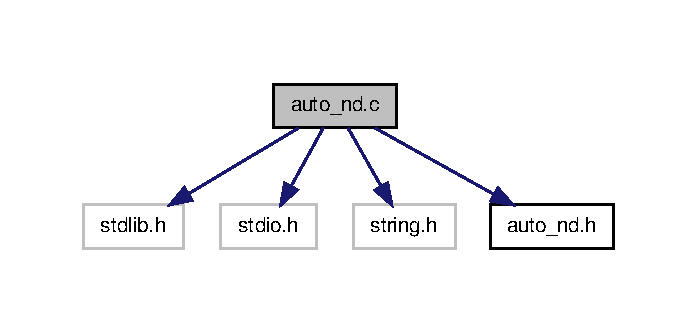
\includegraphics[width=334pt]{auto__nd_8c__incl}
\end{center}
\end{figure}
\subsection*{\-Fonctions}
\begin{DoxyCompactItemize}
\item 
\hyperlink{struct_automate___n_d}{\-Automate\-\_\-\-N\-D} \hyperlink{auto__nd_8c_af69591ffe63ee61cfca113793e74a52a}{auto\-\_\-nd\-\_\-creer} ()
\begin{DoxyCompactList}\small\item\em \-Création d'un automate indéterministe vide. \end{DoxyCompactList}\item 
\hyperlink{struct_automate___n_d}{\-Automate\-\_\-\-N\-D} \hyperlink{auto__nd_8c_aaffcc81be17700a307595e9021d365dd}{auto\-\_\-nd\-\_\-creer\-P} (\hyperlink{auto__nd_8h_a8a9f3c362f156e37cdf72bfac024d7e3}{\-Ensemble\-Char} s, \hyperlink{auto__nd_8h_ab97da0c1b1e5f14d8f0cec086e90fece}{\-Ets} e, \hyperlink{auto__nd_8h_ab97da0c1b1e5f14d8f0cec086e90fece}{\-Ets} i, \hyperlink{auto__nd_8h_ab97da0c1b1e5f14d8f0cec086e90fece}{\-Ets} f, \hyperlink{auto__nd_8h_abefd29f277cc57fe5d7540dcfa9c9edc}{\-Ensemble\-Transition} d)
\begin{DoxyCompactList}\small\item\em \-Création d'un automate indéterministe non vide. \end{DoxyCompactList}\item 
int \hyperlink{auto__nd_8c_a27230e67e659bac8ff1df31d275b51d7}{auto\-\_\-nd\-\_\-detruire} (\hyperlink{struct_automate___n_d}{\-Automate\-\_\-\-N\-D} auto\-\_\-nd)
\begin{DoxyCompactList}\small\item\em \-Destruction d'un automate indéterministe. \end{DoxyCompactList}\item 
\hyperlink{struct_automate___n_d}{\-Automate\-\_\-\-N\-D} \hyperlink{auto__nd_8c_a212359ae461e94794fe0c56881505be5}{auto\-\_\-nd\-\_\-clone} (\hyperlink{struct_automate___n_d}{\-Automate\-\_\-\-N\-D} auto\-\_\-nd)
\begin{DoxyCompactList}\small\item\em \-Clonage d'un automate indéterministe. \end{DoxyCompactList}\item 
\hyperlink{auto__nd_8h_a04b323d3d7ddb72161c7d0a8ba6b20b6}{\-Chaine} \hyperlink{auto__nd_8c_a0b4c03d4ca0c54f969aa619b017294cd}{auto\-\_\-nd\-\_\-chaine} (\hyperlink{struct_automate___n_d}{\-Automate\-\_\-\-N\-D} auto\-\_\-nd)
\begin{DoxyCompactList}\small\item\em \-Description d'un automate indéterministe. \end{DoxyCompactList}\item 
int \hyperlink{auto__nd_8c_a27515409d8bce85f300634555e05e763}{auto\-\_\-nd\-\_\-appartient} (char $\ast$mot, \hyperlink{struct_automate___n_d}{\-Automate\-\_\-\-N\-D} auto\-\_\-nd)
\begin{DoxyCompactList}\small\item\em \-Test d'appartenance d'un mot au langage d'un automate indéterministe. \end{DoxyCompactList}\item 
int \hyperlink{auto__nd_8c_a79d94e6387dfdcf608f4725352d79f94}{auto\-\_\-nd\-\_\-accessible} (\hyperlink{auto__nd_8h_aae0c86cf5eb18ae170b50062873cb0c1}{\-Etat} e, \hyperlink{struct_automate___n_d}{\-Automate\-\_\-\-N\-D} auto\-\_\-nd)
\begin{DoxyCompactList}\small\item\em \-Test d'accessibilité d'un état d'un automate indéterministe. \end{DoxyCompactList}\item 
int \hyperlink{auto__nd_8c_afe137460d216b118270adf740722bd27}{auto\-\_\-nd\-\_\-coaccessible} (\hyperlink{auto__nd_8h_aae0c86cf5eb18ae170b50062873cb0c1}{\-Etat} e, \hyperlink{struct_automate___n_d}{\-Automate\-\_\-\-N\-D} auto\-\_\-nd)
\begin{DoxyCompactList}\small\item\em \-Test de co-\/accessibilité d'un état d'un automate indéterministe. \end{DoxyCompactList}\item 
int \hyperlink{auto__nd_8c_a3f3692af6a52ea59d2fb11706aa0e5b3}{auto\-\_\-nd\-\_\-jumeaux} (\hyperlink{struct_automate___n_d}{\-Automate\-\_\-\-N\-D} auto\-\_\-nd1, \hyperlink{struct_automate___n_d}{\-Automate\-\_\-\-N\-D} auto\-\_\-nd2)
\begin{DoxyCompactList}\small\item\em \-Test de gémélité (clone) entre deux automates indéterministes. \end{DoxyCompactList}\item 
int \hyperlink{auto__nd_8c_a3f519dfe982a416e1817ad4baf7b6370}{auto\-\_\-nd\-\_\-equivalents} (\hyperlink{struct_automate___n_d}{\-Automate\-\_\-\-N\-D} auto\-\_\-nd1, \hyperlink{struct_automate___n_d}{\-Automate\-\_\-\-N\-D} auto\-\_\-nd2)
\begin{DoxyCompactList}\small\item\em \-Test d'équivalence (langage) de deux automates indéterministes. \end{DoxyCompactList}\item 
int \hyperlink{auto__nd_8c_a1a3c107277000a6257a89a8480ee1afd}{auto\-\_\-nd\-\_\-nb\-Lettres} (\hyperlink{struct_automate___n_d}{\-Automate\-\_\-\-N\-D} auto\-\_\-nd)
\begin{DoxyCompactList}\small\item\em \-Nombre de lettre de l'alphabet d'un automate indéterministe. \end{DoxyCompactList}\item 
int \hyperlink{auto__nd_8c_a61fe4e60e7bc060738643fd05c8932a0}{auto\-\_\-nd\-\_\-nb\-Etats} (\hyperlink{struct_automate___n_d}{\-Automate\-\_\-\-N\-D} auto\-\_\-nd)
\begin{DoxyCompactList}\small\item\em \-Nombre d'états total d'un automate indéterministe. \end{DoxyCompactList}\item 
int \hyperlink{auto__nd_8c_a31a554bb355b78f8c9650e0ad2494619}{auto\-\_\-nd\-\_\-nb\-Initiaux} (\hyperlink{struct_automate___n_d}{\-Automate\-\_\-\-N\-D} auto\-\_\-nd)
\begin{DoxyCompactList}\small\item\em \-Nombre d'états initiaux d'un automate indéterministe. \end{DoxyCompactList}\item 
int \hyperlink{auto__nd_8c_a6a77bca76f0c078d5c77a7d58ae1f680}{auto\-\_\-nd\-\_\-nb\-Finaux} (\hyperlink{struct_automate___n_d}{\-Automate\-\_\-\-N\-D} auto\-\_\-nd)
\begin{DoxyCompactList}\small\item\em \-Nombre d'états finaux d'un automate indéterministe. \end{DoxyCompactList}\item 
int \hyperlink{auto__nd_8c_a377f0d84c496692b423d7df61fa2d85a}{auto\-\_\-nd\-\_\-nb\-Transitions} (\hyperlink{struct_automate___n_d}{\-Automate\-\_\-\-N\-D} auto\-\_\-nd)
\begin{DoxyCompactList}\small\item\em \-Nombre de transitions d'un automate indéterministe. \end{DoxyCompactList}\item 
void \hyperlink{auto__nd_8c_a684e405d2bcaaeaab6309221f92ee5a6}{auto\-\_\-nd\-\_\-ajout\-Lettre} (char c, \hyperlink{struct_automate___n_d}{\-Automate\-\_\-\-N\-D} auto\-\_\-nd)
\begin{DoxyCompactList}\small\item\em \-Ajoute une lettre \-A\-S\-C\-I\-I à l'alphabet d'un automate indéterministe. \end{DoxyCompactList}\item 
void \hyperlink{auto__nd_8c_a699f7374d01be804c5d5a0f2d8ee8872}{auto\-\_\-nd\-\_\-ajout\-Etat} (\hyperlink{auto__nd_8h_aae0c86cf5eb18ae170b50062873cb0c1}{\-Etat} e, \hyperlink{struct_automate___n_d}{\-Automate\-\_\-\-N\-D} auto\-\_\-nd)
\begin{DoxyCompactList}\small\item\em \-Ajoute un état (non initial, non final) à un automate indéterministe. \end{DoxyCompactList}\item 
void \hyperlink{auto__nd_8c_ae290407f1418df8dd0cb1a612901ae37}{auto\-\_\-nd\-\_\-ajout\-Initial} (\hyperlink{auto__nd_8h_aae0c86cf5eb18ae170b50062873cb0c1}{\-Etat} i, \hyperlink{struct_automate___n_d}{\-Automate\-\_\-\-N\-D} auto\-\_\-nd)
\begin{DoxyCompactList}\small\item\em \-Ajoute un état initial à un automate indéterministe. \end{DoxyCompactList}\item 
void \hyperlink{auto__nd_8c_ad92ce4c86d5d4f695e614eba93a90c82}{auto\-\_\-nd\-\_\-ajout\-Final} (\hyperlink{auto__nd_8h_aae0c86cf5eb18ae170b50062873cb0c1}{\-Etat} f, \hyperlink{struct_automate___n_d}{\-Automate\-\_\-\-N\-D} auto\-\_\-nd)
\begin{DoxyCompactList}\small\item\em \-Ajoute un état final à un automate indéterministe. \end{DoxyCompactList}\item 
void \hyperlink{auto__nd_8c_ab4389b9b99010af37b0a1f55ba565a35}{auto\-\_\-nd\-\_\-ajout\-Transition} (\hyperlink{struct_transition}{\-Transition} t, \hyperlink{struct_automate___n_d}{\-Automate\-\_\-\-N\-D} auto\-\_\-nd)
\begin{DoxyCompactList}\small\item\em \-Ajoute une transition à un automate indéterministe. \end{DoxyCompactList}\item 
void \hyperlink{auto__nd_8c_a71fd5b027c59c569247c144a97aac72f}{auto\-\_\-nd\-\_\-suppr\-Lettre} (char c, \hyperlink{struct_automate___n_d}{\-Automate\-\_\-\-N\-D} auto\-\_\-nd)
\begin{DoxyCompactList}\small\item\em \-Retire une lettre \-A\-S\-C\-I\-I à l'alphabet d'un automate indéterministe. \end{DoxyCompactList}\item 
void \hyperlink{auto__nd_8c_abc8e956fda2f30bc3af985a4a002a5ee}{auto\-\_\-nd\-\_\-suppr\-Etat} (\hyperlink{auto__nd_8h_aae0c86cf5eb18ae170b50062873cb0c1}{\-Etat} e, \hyperlink{struct_automate___n_d}{\-Automate\-\_\-\-N\-D} auto\-\_\-nd)
\begin{DoxyCompactList}\small\item\em \-Retire un état à un automate indéterministe. \end{DoxyCompactList}\item 
void \hyperlink{auto__nd_8c_aca2642240007ce7acab36a6ddc994a69}{auto\-\_\-nd\-\_\-suppr\-Transition} (\hyperlink{struct_transition}{\-Transition} t, \hyperlink{struct_automate___n_d}{\-Automate\-\_\-\-N\-D} auto\-\_\-nd)
\begin{DoxyCompactList}\small\item\em \-Retire une transition à un automate indéterministe. \end{DoxyCompactList}\item 
\hyperlink{struct_automate___n_d}{\-Automate\-\_\-\-N\-D} \hyperlink{auto__nd_8c_a5bd71be0cb8a4c522c1ee818496983c5}{auto\-\_\-nd\-\_\-completer} (\hyperlink{struct_automate___n_d}{\-Automate\-\_\-\-N\-D} auto\-\_\-nd)
\begin{DoxyCompactList}\small\item\em \-Complète un automate indéterministe. \end{DoxyCompactList}\item 
\hyperlink{struct_automate___n_d}{\-Automate\-\_\-\-N\-D} \hyperlink{auto__nd_8c_a2649a06ebe3a71986c20371c16465636}{auto\-\_\-nd\-\_\-reduire} (\hyperlink{struct_automate___n_d}{\-Automate\-\_\-\-N\-D} auto\-\_\-nd)
\begin{DoxyCompactList}\small\item\em \-Réduit un automate indéterministe. \end{DoxyCompactList}\item 
\hyperlink{auto__nd_8h_a04b323d3d7ddb72161c7d0a8ba6b20b6}{\-Chaine} \hyperlink{auto__nd_8c_a956166e9403f28b1544dbc475db7afee}{auto\-\_\-nd\-\_\-liste\-Mots} (int debut, int fin, \hyperlink{struct_automate___n_d}{\-Automate\-\_\-\-N\-D} auto\-\_\-nd)
\begin{DoxyCompactList}\small\item\em \-Liste les mots (suivant une fourchette de longueur) appartenants au langage d'un automate indéterministe. \end{DoxyCompactList}\item 
\hyperlink{auto__nd_8h_a04b323d3d7ddb72161c7d0a8ba6b20b6}{\-Chaine} \hyperlink{auto__nd_8c_aa18a4077a0868825391d5737fa0c8d29}{auto\-\_\-nd\-\_\-liste\-Mots\-Alpha} (int debut, int fin, \hyperlink{struct_automate___n_d}{\-Automate\-\_\-\-N\-D} auto\-\_\-nd)
\begin{DoxyCompactList}\small\item\em \-Liste lexicographiquement les mots (suivant une fourchette de longueur) appartenants au langage d'un automate indéterministe. \end{DoxyCompactList}\item 
\hyperlink{auto__nd_8h_a04b323d3d7ddb72161c7d0a8ba6b20b6}{\-Chaine} \hyperlink{auto__nd_8c_a269f375009f4853e3f08f38142dbb2e2}{auto\-\_\-nd\-\_\-chemin} (char $\ast$mot, \hyperlink{struct_automate___n_d}{\-Automate\-\_\-\-N\-D} auto\-\_\-nd)
\begin{DoxyCompactList}\small\item\em \-Fourni un chemin possible d'un mot pour un automate indéterministe donné. \end{DoxyCompactList}\item 
\hyperlink{auto__nd_8h_a04b323d3d7ddb72161c7d0a8ba6b20b6}{\-Chaine} \hyperlink{auto__nd_8c_a8b25b03f74ee27486bbe15f29c9d5aa7}{auto\-\_\-nd\-\_\-chemins} (char $\ast$mot, \hyperlink{struct_automate___n_d}{\-Automate\-\_\-\-N\-D} auto\-\_\-nd)
\begin{DoxyCompactList}\small\item\em \-Fourni la liste de tous les chemins possible d'un mot pour un automate indéterministe donné. \end{DoxyCompactList}\item 
int \hyperlink{auto__nd_8c_ad2d27eb4a14392cbb539d56d41524318}{auto\-\_\-nd\-\_\-nb\-Chemins\-Possibles} (char $\ast$mot, \hyperlink{struct_automate___n_d}{\-Automate\-\_\-\-N\-D} auto\-\_\-nd)
\begin{DoxyCompactList}\small\item\em \-Nombre de chemins possibles d'un mot pour un automate indéterministe donné. \end{DoxyCompactList}\end{DoxyCompactItemize}


\subsection{\-Description détaillée}
\-Code des \-Automates indéterministes. \begin{DoxyAuthor}{\-Auteur}
\-Gauthier \-Silvère
\end{DoxyAuthor}
\-Fichier d'implémentation fonctions concernant les automates indéterministes. 

\-Définition dans le fichier \hyperlink{auto__nd_8c_source}{auto\-\_\-nd.\-c}.



\subsection{\-Documentation des fonctions}
\hypertarget{auto__nd_8c_a79d94e6387dfdcf608f4725352d79f94}{\index{auto\-\_\-nd.\-c@{auto\-\_\-nd.\-c}!auto\-\_\-nd\-\_\-accessible@{auto\-\_\-nd\-\_\-accessible}}
\index{auto\-\_\-nd\-\_\-accessible@{auto\-\_\-nd\-\_\-accessible}!auto_nd.c@{auto\-\_\-nd.\-c}}
\subsubsection[{auto\-\_\-nd\-\_\-accessible}]{\setlength{\rightskip}{0pt plus 5cm}int {\bf auto\-\_\-nd\-\_\-accessible} (
\begin{DoxyParamCaption}
\item[{{\bf \-Etat}}]{e, }
\item[{{\bf \-Automate\-\_\-\-N\-D}}]{auto\-\_\-nd}
\end{DoxyParamCaption}
)}}\label{auto__nd_8c_a79d94e6387dfdcf608f4725352d79f94}


\-Test d'accessibilité d'un état d'un automate indéterministe. 


\begin{DoxyParams}[1]{\-Paramètres}
\mbox{\tt in}  & {\em e} & \-Etat à tester. \\
\hline
\mbox{\tt in}  & {\em auto\-\_\-nd} & \-Automate sur lequel faire le test. \\
\hline
\end{DoxyParams}
\begin{DoxyReturn}{\-Renvoie}
1 si accessibilité, 0 sinon. 
\end{DoxyReturn}
\hypertarget{auto__nd_8c_a699f7374d01be804c5d5a0f2d8ee8872}{\index{auto\-\_\-nd.\-c@{auto\-\_\-nd.\-c}!auto\-\_\-nd\-\_\-ajout\-Etat@{auto\-\_\-nd\-\_\-ajout\-Etat}}
\index{auto\-\_\-nd\-\_\-ajout\-Etat@{auto\-\_\-nd\-\_\-ajout\-Etat}!auto_nd.c@{auto\-\_\-nd.\-c}}
\subsubsection[{auto\-\_\-nd\-\_\-ajout\-Etat}]{\setlength{\rightskip}{0pt plus 5cm}void {\bf auto\-\_\-nd\-\_\-ajout\-Etat} (
\begin{DoxyParamCaption}
\item[{{\bf \-Etat}}]{e, }
\item[{{\bf \-Automate\-\_\-\-N\-D}}]{auto\-\_\-nd}
\end{DoxyParamCaption}
)}}\label{auto__nd_8c_a699f7374d01be804c5d5a0f2d8ee8872}


\-Ajoute un état (non initial, non final) à un automate indéterministe. 


\begin{DoxyParams}[1]{\-Paramètres}
\mbox{\tt in}  & {\em e} & \-Etat à ajouter. \-Les doublons sont gérés. \\
\hline
\mbox{\tt in,out}  & {\em auto\-\_\-nd} & \-Automate auquel ajouter. \\
\hline
\end{DoxyParams}
\hypertarget{auto__nd_8c_ad92ce4c86d5d4f695e614eba93a90c82}{\index{auto\-\_\-nd.\-c@{auto\-\_\-nd.\-c}!auto\-\_\-nd\-\_\-ajout\-Final@{auto\-\_\-nd\-\_\-ajout\-Final}}
\index{auto\-\_\-nd\-\_\-ajout\-Final@{auto\-\_\-nd\-\_\-ajout\-Final}!auto_nd.c@{auto\-\_\-nd.\-c}}
\subsubsection[{auto\-\_\-nd\-\_\-ajout\-Final}]{\setlength{\rightskip}{0pt plus 5cm}void {\bf auto\-\_\-nd\-\_\-ajout\-Final} (
\begin{DoxyParamCaption}
\item[{{\bf \-Etat}}]{f, }
\item[{{\bf \-Automate\-\_\-\-N\-D}}]{auto\-\_\-nd}
\end{DoxyParamCaption}
)}}\label{auto__nd_8c_ad92ce4c86d5d4f695e614eba93a90c82}


\-Ajoute un état final à un automate indéterministe. 


\begin{DoxyParams}[1]{\-Paramètres}
\mbox{\tt in}  & {\em f} & \-Etat final à ajouter. \-Les doublons sont gérés. \\
\hline
\mbox{\tt in,out}  & {\em auto\-\_\-nd} & \-Automate auquel ajouter. \\
\hline
\end{DoxyParams}
\hypertarget{auto__nd_8c_ae290407f1418df8dd0cb1a612901ae37}{\index{auto\-\_\-nd.\-c@{auto\-\_\-nd.\-c}!auto\-\_\-nd\-\_\-ajout\-Initial@{auto\-\_\-nd\-\_\-ajout\-Initial}}
\index{auto\-\_\-nd\-\_\-ajout\-Initial@{auto\-\_\-nd\-\_\-ajout\-Initial}!auto_nd.c@{auto\-\_\-nd.\-c}}
\subsubsection[{auto\-\_\-nd\-\_\-ajout\-Initial}]{\setlength{\rightskip}{0pt plus 5cm}void {\bf auto\-\_\-nd\-\_\-ajout\-Initial} (
\begin{DoxyParamCaption}
\item[{{\bf \-Etat}}]{i, }
\item[{{\bf \-Automate\-\_\-\-N\-D}}]{auto\-\_\-nd}
\end{DoxyParamCaption}
)}}\label{auto__nd_8c_ae290407f1418df8dd0cb1a612901ae37}


\-Ajoute un état initial à un automate indéterministe. 


\begin{DoxyParams}[1]{\-Paramètres}
\mbox{\tt in}  & {\em i} & \-Etat initial à ajouter. \-Les doublons sont gérés. \\
\hline
\mbox{\tt in,out}  & {\em auto\-\_\-nd} & \-Automate auquel ajouter. \\
\hline
\end{DoxyParams}
\hypertarget{auto__nd_8c_a684e405d2bcaaeaab6309221f92ee5a6}{\index{auto\-\_\-nd.\-c@{auto\-\_\-nd.\-c}!auto\-\_\-nd\-\_\-ajout\-Lettre@{auto\-\_\-nd\-\_\-ajout\-Lettre}}
\index{auto\-\_\-nd\-\_\-ajout\-Lettre@{auto\-\_\-nd\-\_\-ajout\-Lettre}!auto_nd.c@{auto\-\_\-nd.\-c}}
\subsubsection[{auto\-\_\-nd\-\_\-ajout\-Lettre}]{\setlength{\rightskip}{0pt plus 5cm}int {\bf auto\-\_\-nd\-\_\-ajout\-Lettre} (
\begin{DoxyParamCaption}
\item[{char}]{c, }
\item[{{\bf \-Automate\-\_\-\-N\-D}}]{auto\-\_\-nd}
\end{DoxyParamCaption}
)}}\label{auto__nd_8c_a684e405d2bcaaeaab6309221f92ee5a6}


\-Ajoute une lettre \-A\-S\-C\-I\-I à l'alphabet d'un automate indéterministe. 


\begin{DoxyParams}[1]{\-Paramètres}
\mbox{\tt in}  & {\em c} & \-Lettre \-A\-S\-C\-I\-I à ajouter. \-Les doublons sont gérés. \\
\hline
\mbox{\tt in,out}  & {\em auto\-\_\-nd} & \-Automate auquel ajouter. \\
\hline
\end{DoxyParams}
\hypertarget{auto__nd_8c_ab4389b9b99010af37b0a1f55ba565a35}{\index{auto\-\_\-nd.\-c@{auto\-\_\-nd.\-c}!auto\-\_\-nd\-\_\-ajout\-Transition@{auto\-\_\-nd\-\_\-ajout\-Transition}}
\index{auto\-\_\-nd\-\_\-ajout\-Transition@{auto\-\_\-nd\-\_\-ajout\-Transition}!auto_nd.c@{auto\-\_\-nd.\-c}}
\subsubsection[{auto\-\_\-nd\-\_\-ajout\-Transition}]{\setlength{\rightskip}{0pt plus 5cm}void {\bf auto\-\_\-nd\-\_\-ajout\-Transition} (
\begin{DoxyParamCaption}
\item[{{\bf \-Transition}}]{t, }
\item[{{\bf \-Automate\-\_\-\-N\-D}}]{auto\-\_\-nd}
\end{DoxyParamCaption}
)}}\label{auto__nd_8c_ab4389b9b99010af37b0a1f55ba565a35}


\-Ajoute une transition à un automate indéterministe. 


\begin{DoxyParams}[1]{\-Paramètres}
\mbox{\tt in}  & {\em t} & \hyperlink{struct_transition}{\-Transition} à ajouter. \-Les doublons sont gérés. \\
\hline
\mbox{\tt in,out}  & {\em auto\-\_\-nd} & \-Automate auquel ajouter. \\
\hline
\end{DoxyParams}
\hypertarget{auto__nd_8c_a27515409d8bce85f300634555e05e763}{\index{auto\-\_\-nd.\-c@{auto\-\_\-nd.\-c}!auto\-\_\-nd\-\_\-appartient@{auto\-\_\-nd\-\_\-appartient}}
\index{auto\-\_\-nd\-\_\-appartient@{auto\-\_\-nd\-\_\-appartient}!auto_nd.c@{auto\-\_\-nd.\-c}}
\subsubsection[{auto\-\_\-nd\-\_\-appartient}]{\setlength{\rightskip}{0pt plus 5cm}int {\bf auto\-\_\-nd\-\_\-appartient} (
\begin{DoxyParamCaption}
\item[{char $\ast$}]{mot, }
\item[{{\bf \-Automate\-\_\-\-N\-D}}]{auto\-\_\-nd}
\end{DoxyParamCaption}
)}}\label{auto__nd_8c_a27515409d8bce85f300634555e05e763}


\-Test d'appartenance d'un mot au langage d'un automate indéterministe. 


\begin{DoxyParams}[1]{\-Paramètres}
\mbox{\tt in}  & {\em mot} & \-Mot à tester. \\
\hline
\mbox{\tt in}  & {\em auto\-\_\-nd} & \-Automate sur lequel faire le test. \\
\hline
\end{DoxyParams}
\begin{DoxyReturn}{\-Renvoie}
1 si appartenance, 0 sinon. 
\end{DoxyReturn}
\hypertarget{auto__nd_8c_a0b4c03d4ca0c54f969aa619b017294cd}{\index{auto\-\_\-nd.\-c@{auto\-\_\-nd.\-c}!auto\-\_\-nd\-\_\-chaine@{auto\-\_\-nd\-\_\-chaine}}
\index{auto\-\_\-nd\-\_\-chaine@{auto\-\_\-nd\-\_\-chaine}!auto_nd.c@{auto\-\_\-nd.\-c}}
\subsubsection[{auto\-\_\-nd\-\_\-chaine}]{\setlength{\rightskip}{0pt plus 5cm}{\bf \-Chaine} {\bf auto\-\_\-nd\-\_\-chaine} (
\begin{DoxyParamCaption}
\item[{{\bf \-Automate\-\_\-\-N\-D}}]{auto\-\_\-nd}
\end{DoxyParamCaption}
)}}\label{auto__nd_8c_a0b4c03d4ca0c54f969aa619b017294cd}


\-Description d'un automate indéterministe. 


\begin{DoxyParams}[1]{\-Paramètres}
\mbox{\tt in}  & {\em auto\-\_\-nd} & \-Automate à décrire. \\
\hline
\end{DoxyParams}
\begin{DoxyReturn}{\-Renvoie}
\-Chaîne de caractères décrivant l'automate indéterministe passé en paramètre. 
\end{DoxyReturn}


\-Définition à la ligne 50 du fichier auto\-\_\-nd.\-c.

\hypertarget{auto__nd_8c_a269f375009f4853e3f08f38142dbb2e2}{\index{auto\-\_\-nd.\-c@{auto\-\_\-nd.\-c}!auto\-\_\-nd\-\_\-chemin@{auto\-\_\-nd\-\_\-chemin}}
\index{auto\-\_\-nd\-\_\-chemin@{auto\-\_\-nd\-\_\-chemin}!auto_nd.c@{auto\-\_\-nd.\-c}}
\subsubsection[{auto\-\_\-nd\-\_\-chemin}]{\setlength{\rightskip}{0pt plus 5cm}{\bf \-Chaine} {\bf auto\-\_\-nd\-\_\-chemin} (
\begin{DoxyParamCaption}
\item[{char $\ast$}]{mot, }
\item[{{\bf \-Automate\-\_\-\-N\-D}}]{auto\-\_\-nd}
\end{DoxyParamCaption}
)}}\label{auto__nd_8c_a269f375009f4853e3f08f38142dbb2e2}


\-Fourni un chemin possible d'un mot pour un automate indéterministe donné. 


\begin{DoxyParams}[1]{\-Paramètres}
\mbox{\tt in}  & {\em mot} & \-Chaine de caractères \-A\-S\-C\-I\-I à tester. \\
\hline
\mbox{\tt in}  & {\em auto\-\_\-nd} & \-Automate à interroger. \\
\hline
\end{DoxyParams}
\begin{DoxyReturn}{\-Renvoie}
\-Une chaine de caractères correspondant au chemin parcouru, s'il existe. \-N\-U\-L\-L sinon. 
\end{DoxyReturn}
\hypertarget{auto__nd_8c_a8b25b03f74ee27486bbe15f29c9d5aa7}{\index{auto\-\_\-nd.\-c@{auto\-\_\-nd.\-c}!auto\-\_\-nd\-\_\-chemins@{auto\-\_\-nd\-\_\-chemins}}
\index{auto\-\_\-nd\-\_\-chemins@{auto\-\_\-nd\-\_\-chemins}!auto_nd.c@{auto\-\_\-nd.\-c}}
\subsubsection[{auto\-\_\-nd\-\_\-chemins}]{\setlength{\rightskip}{0pt plus 5cm}{\bf \-Chaine} {\bf auto\-\_\-nd\-\_\-chemins} (
\begin{DoxyParamCaption}
\item[{char $\ast$}]{mot, }
\item[{{\bf \-Automate\-\_\-\-N\-D}}]{auto\-\_\-nd}
\end{DoxyParamCaption}
)}}\label{auto__nd_8c_a8b25b03f74ee27486bbe15f29c9d5aa7}


\-Fourni la liste de tous les chemins possible d'un mot pour un automate indéterministe donné. 


\begin{DoxyParams}[1]{\-Paramètres}
\mbox{\tt in}  & {\em mot} & \-Chaine de caractères \-A\-S\-C\-I\-I à tester. \\
\hline
\mbox{\tt in}  & {\em auto\-\_\-nd} & \-Automate à interroger. \\
\hline
\end{DoxyParams}
\begin{DoxyReturn}{\-Renvoie}
\-Une chaine de caractères correspondant à la liste des chemins parcourus, s'ils existent. \-N\-U\-L\-L sinon. 
\end{DoxyReturn}
\hypertarget{auto__nd_8c_a212359ae461e94794fe0c56881505be5}{\index{auto\-\_\-nd.\-c@{auto\-\_\-nd.\-c}!auto\-\_\-nd\-\_\-clone@{auto\-\_\-nd\-\_\-clone}}
\index{auto\-\_\-nd\-\_\-clone@{auto\-\_\-nd\-\_\-clone}!auto_nd.c@{auto\-\_\-nd.\-c}}
\subsubsection[{auto\-\_\-nd\-\_\-clone}]{\setlength{\rightskip}{0pt plus 5cm}{\bf \-Automate\-\_\-\-N\-D} {\bf auto\-\_\-nd\-\_\-clone} (
\begin{DoxyParamCaption}
\item[{{\bf \-Automate\-\_\-\-N\-D}}]{auto\-\_\-nd}
\end{DoxyParamCaption}
)}}\label{auto__nd_8c_a212359ae461e94794fe0c56881505be5}


\-Clonage d'un automate indéterministe. 


\begin{DoxyParams}[1]{\-Paramètres}
\mbox{\tt in}  & {\em auto\-\_\-nd} & \-Automate à cloner. \\
\hline
\end{DoxyParams}
\begin{DoxyReturn}{\-Renvoie}
\-Instance nouvelle d'un \hyperlink{struct_automate___n_d}{\-Automate\-\_\-\-N\-D} alloué d'ensembles identiques à auto\-\_\-nd (par copie). 
\end{DoxyReturn}


\-Définition à la ligne 46 du fichier auto\-\_\-nd.\-c.

\hypertarget{auto__nd_8c_afe137460d216b118270adf740722bd27}{\index{auto\-\_\-nd.\-c@{auto\-\_\-nd.\-c}!auto\-\_\-nd\-\_\-coaccessible@{auto\-\_\-nd\-\_\-coaccessible}}
\index{auto\-\_\-nd\-\_\-coaccessible@{auto\-\_\-nd\-\_\-coaccessible}!auto_nd.c@{auto\-\_\-nd.\-c}}
\subsubsection[{auto\-\_\-nd\-\_\-coaccessible}]{\setlength{\rightskip}{0pt plus 5cm}int {\bf auto\-\_\-nd\-\_\-coaccessible} (
\begin{DoxyParamCaption}
\item[{{\bf \-Etat}}]{e, }
\item[{{\bf \-Automate\-\_\-\-N\-D}}]{auto\-\_\-nd}
\end{DoxyParamCaption}
)}}\label{auto__nd_8c_afe137460d216b118270adf740722bd27}


\-Test de co-\/accessibilité d'un état d'un automate indéterministe. 


\begin{DoxyParams}[1]{\-Paramètres}
\mbox{\tt in}  & {\em e} & \-Etat à tester. \\
\hline
\mbox{\tt in}  & {\em auto\-\_\-nd} & \-Automate sur lequel faire le test. \\
\hline
\end{DoxyParams}
\begin{DoxyReturn}{\-Renvoie}
1 si co-\/accessibilité, 0 sinon. 
\end{DoxyReturn}
\hypertarget{auto__nd_8c_a5bd71be0cb8a4c522c1ee818496983c5}{\index{auto\-\_\-nd.\-c@{auto\-\_\-nd.\-c}!auto\-\_\-nd\-\_\-completer@{auto\-\_\-nd\-\_\-completer}}
\index{auto\-\_\-nd\-\_\-completer@{auto\-\_\-nd\-\_\-completer}!auto_nd.c@{auto\-\_\-nd.\-c}}
\subsubsection[{auto\-\_\-nd\-\_\-completer}]{\setlength{\rightskip}{0pt plus 5cm}{\bf \-Automate\-\_\-\-N\-D} {\bf auto\-\_\-nd\-\_\-completer} (
\begin{DoxyParamCaption}
\item[{{\bf \-Automate\-\_\-\-N\-D}}]{auto\-\_\-nd}
\end{DoxyParamCaption}
)}}\label{auto__nd_8c_a5bd71be0cb8a4c522c1ee818496983c5}


\-Complète un automate indéterministe. 


\begin{DoxyParams}[1]{\-Paramètres}
\mbox{\tt in}  & {\em auto\-\_\-nd} & \-Automate à compléter. \-Peut être complet. \\
\hline
\end{DoxyParams}
\begin{DoxyReturn}{\-Renvoie}
\-Un \hyperlink{struct_automate___n_d}{\-Automate\-\_\-\-N\-D} correspondant à l'automate paramètre complété. 
\end{DoxyReturn}
\hypertarget{auto__nd_8c_af69591ffe63ee61cfca113793e74a52a}{\index{auto\-\_\-nd.\-c@{auto\-\_\-nd.\-c}!auto\-\_\-nd\-\_\-creer@{auto\-\_\-nd\-\_\-creer}}
\index{auto\-\_\-nd\-\_\-creer@{auto\-\_\-nd\-\_\-creer}!auto_nd.c@{auto\-\_\-nd.\-c}}
\subsubsection[{auto\-\_\-nd\-\_\-creer}]{\setlength{\rightskip}{0pt plus 5cm}{\bf \-Automate\-\_\-\-N\-D} {\bf auto\-\_\-nd\-\_\-creer} (
\begin{DoxyParamCaption}
{}
\end{DoxyParamCaption}
)}}\label{auto__nd_8c_af69591ffe63ee61cfca113793e74a52a}


\-Création d'un automate indéterministe vide. 

\begin{DoxyReturn}{\-Renvoie}
\-Instance nouvelle d'un \hyperlink{struct_automate___n_d}{\-Automate\-\_\-\-N\-D} alloué d'ensembles vides. 
\end{DoxyReturn}


\-Définition à la ligne 18 du fichier auto\-\_\-nd.\-c.

\hypertarget{auto__nd_8c_aaffcc81be17700a307595e9021d365dd}{\index{auto\-\_\-nd.\-c@{auto\-\_\-nd.\-c}!auto\-\_\-nd\-\_\-creer\-P@{auto\-\_\-nd\-\_\-creer\-P}}
\index{auto\-\_\-nd\-\_\-creer\-P@{auto\-\_\-nd\-\_\-creer\-P}!auto_nd.c@{auto\-\_\-nd.\-c}}
\subsubsection[{auto\-\_\-nd\-\_\-creer\-P}]{\setlength{\rightskip}{0pt plus 5cm}{\bf \-Automate\-\_\-\-N\-D} {\bf auto\-\_\-nd\-\_\-creer\-P} (
\begin{DoxyParamCaption}
\item[{{\bf \-Ensemble\-Char}}]{s, }
\item[{{\bf \-Ets}}]{e, }
\item[{{\bf \-Ets}}]{i, }
\item[{{\bf \-Ets}}]{f, }
\item[{{\bf \-Ensemble\-Transition}}]{d}
\end{DoxyParamCaption}
)}}\label{auto__nd_8c_aaffcc81be17700a307595e9021d365dd}


\-Création d'un automate indéterministe non vide. 


\begin{DoxyParams}[1]{\-Paramètres}
\mbox{\tt in}  & {\em s} & \-Alphabet sigma. \-Peux être vide. \\
\hline
\mbox{\tt in}  & {\em e} & \-Ensemble total d'états \-E. \-Peux être vide. \\
\hline
\mbox{\tt in}  & {\em i} & pour \-I. \-Peux être vide. \\
\hline
\mbox{\tt in}  & {\em f} & pour \-F. \-Peux être vide. \\
\hline
\mbox{\tt in}  & {\em d} & pour delta. \-Peux être vide. \\
\hline
\end{DoxyParams}
\begin{DoxyReturn}{\-Renvoie}
\-Instance nouvelle d'un \hyperlink{struct_automate___n_d}{\-Automate\-\_\-\-N\-D} alloué des ensembles passés en paramètres. 
\end{DoxyReturn}


\-Définition à la ligne 28 du fichier auto\-\_\-nd.\-c.

\hypertarget{auto__nd_8c_a27230e67e659bac8ff1df31d275b51d7}{\index{auto\-\_\-nd.\-c@{auto\-\_\-nd.\-c}!auto\-\_\-nd\-\_\-detruire@{auto\-\_\-nd\-\_\-detruire}}
\index{auto\-\_\-nd\-\_\-detruire@{auto\-\_\-nd\-\_\-detruire}!auto_nd.c@{auto\-\_\-nd.\-c}}
\subsubsection[{auto\-\_\-nd\-\_\-detruire}]{\setlength{\rightskip}{0pt plus 5cm}{\bf auto\-\_\-nd\-\_\-detruire} (
\begin{DoxyParamCaption}
\item[{{\bf \-Automate\-\_\-\-N\-D}}]{auto\-\_\-nd}
\end{DoxyParamCaption}
)}}\label{auto__nd_8c_a27230e67e659bac8ff1df31d275b51d7}


\-Destruction d'un automate indéterministe. 


\begin{DoxyParams}[1]{\-Paramètres}
\mbox{\tt in,out}  & {\em auto\-\_\-nd} & \-Automate à détruire. \\
\hline
\end{DoxyParams}
\begin{DoxyReturn}{\-Renvoie}
0 si aucune erreur, 1 sinon. 
\end{DoxyReturn}


\-Définition à la ligne 38 du fichier auto\-\_\-nd.\-c.

\hypertarget{auto__nd_8c_a3f519dfe982a416e1817ad4baf7b6370}{\index{auto\-\_\-nd.\-c@{auto\-\_\-nd.\-c}!auto\-\_\-nd\-\_\-equivalents@{auto\-\_\-nd\-\_\-equivalents}}
\index{auto\-\_\-nd\-\_\-equivalents@{auto\-\_\-nd\-\_\-equivalents}!auto_nd.c@{auto\-\_\-nd.\-c}}
\subsubsection[{auto\-\_\-nd\-\_\-equivalents}]{\setlength{\rightskip}{0pt plus 5cm}int {\bf auto\-\_\-nd\-\_\-equivalents} (
\begin{DoxyParamCaption}
\item[{{\bf \-Automate\-\_\-\-N\-D}}]{auto\-\_\-nd1, }
\item[{{\bf \-Automate\-\_\-\-N\-D}}]{auto\-\_\-nd2}
\end{DoxyParamCaption}
)}}\label{auto__nd_8c_a3f519dfe982a416e1817ad4baf7b6370}


\-Test d'équivalence (langage) de deux automates indéterministes. 


\begin{DoxyParams}[1]{\-Paramètres}
\mbox{\tt in}  & {\em auto\-\_\-nd1} & \-Premier automate à tester. \\
\hline
\mbox{\tt in}  & {\em auto\-\_\-nd2} & \-Deuxième automate à tester. \\
\hline
\end{DoxyParams}
\begin{DoxyReturn}{\-Renvoie}
1 si équivalence, 0 sinon. 
\end{DoxyReturn}
\hypertarget{auto__nd_8c_a3f3692af6a52ea59d2fb11706aa0e5b3}{\index{auto\-\_\-nd.\-c@{auto\-\_\-nd.\-c}!auto\-\_\-nd\-\_\-jumeaux@{auto\-\_\-nd\-\_\-jumeaux}}
\index{auto\-\_\-nd\-\_\-jumeaux@{auto\-\_\-nd\-\_\-jumeaux}!auto_nd.c@{auto\-\_\-nd.\-c}}
\subsubsection[{auto\-\_\-nd\-\_\-jumeaux}]{\setlength{\rightskip}{0pt plus 5cm}int {\bf auto\-\_\-nd\-\_\-jumeaux} (
\begin{DoxyParamCaption}
\item[{{\bf \-Automate\-\_\-\-N\-D}}]{auto\-\_\-nd1, }
\item[{{\bf \-Automate\-\_\-\-N\-D}}]{auto\-\_\-nd2}
\end{DoxyParamCaption}
)}}\label{auto__nd_8c_a3f3692af6a52ea59d2fb11706aa0e5b3}


\-Test de gémélité (clone) entre deux automates indéterministes. 


\begin{DoxyParams}[1]{\-Paramètres}
\mbox{\tt in}  & {\em auto\-\_\-nd1} & \-Premier automate à tester. \\
\hline
\mbox{\tt in}  & {\em auto\-\_\-nd2} & \-Deuxième automate à tester. \\
\hline
\end{DoxyParams}
\begin{DoxyReturn}{\-Renvoie}
1 si gémélité, 0 sinon. 
\end{DoxyReturn}
\hypertarget{auto__nd_8c_a956166e9403f28b1544dbc475db7afee}{\index{auto\-\_\-nd.\-c@{auto\-\_\-nd.\-c}!auto\-\_\-nd\-\_\-liste\-Mots@{auto\-\_\-nd\-\_\-liste\-Mots}}
\index{auto\-\_\-nd\-\_\-liste\-Mots@{auto\-\_\-nd\-\_\-liste\-Mots}!auto_nd.c@{auto\-\_\-nd.\-c}}
\subsubsection[{auto\-\_\-nd\-\_\-liste\-Mots}]{\setlength{\rightskip}{0pt plus 5cm}{\bf \-Chaine} {\bf auto\-\_\-nd\-\_\-liste\-Mots} (
\begin{DoxyParamCaption}
\item[{int}]{debut, }
\item[{int}]{fin, }
\item[{{\bf \-Automate\-\_\-\-N\-D}}]{auto\-\_\-nd}
\end{DoxyParamCaption}
)}}\label{auto__nd_8c_a956166e9403f28b1544dbc475db7afee}


\-Liste les mots (suivant une fourchette de longueur) appartenants au langage d'un automate indéterministe. 


\begin{DoxyParams}[1]{\-Paramètres}
\mbox{\tt in}  & {\em debut} & \-Nombre minimal de lettres \-A\-S\-C\-I\-I. \-Doit être positif. \\
\hline
\mbox{\tt in}  & {\em fin} & \-Nombre maximal de lettres \-A\-S\-C\-I\-I. \-Doit être positif et supérieur à début. \\
\hline
\mbox{\tt in}  & {\em auto\-\_\-nd} & \-Automate à interroger. \\
\hline
\end{DoxyParams}
\begin{DoxyReturn}{\-Renvoie}
\-Une chaîne de caractères correspondant à la liste des mots de longueur 'debut' à longueur 'fin'. 
\end{DoxyReturn}
\hypertarget{auto__nd_8c_aa18a4077a0868825391d5737fa0c8d29}{\index{auto\-\_\-nd.\-c@{auto\-\_\-nd.\-c}!auto\-\_\-nd\-\_\-liste\-Mots\-Alpha@{auto\-\_\-nd\-\_\-liste\-Mots\-Alpha}}
\index{auto\-\_\-nd\-\_\-liste\-Mots\-Alpha@{auto\-\_\-nd\-\_\-liste\-Mots\-Alpha}!auto_nd.c@{auto\-\_\-nd.\-c}}
\subsubsection[{auto\-\_\-nd\-\_\-liste\-Mots\-Alpha}]{\setlength{\rightskip}{0pt plus 5cm}{\bf \-Chaine} {\bf auto\-\_\-nd\-\_\-liste\-Mots\-Alpha} (
\begin{DoxyParamCaption}
\item[{int}]{debut, }
\item[{int}]{fin, }
\item[{{\bf \-Automate\-\_\-\-N\-D}}]{auto\-\_\-nd}
\end{DoxyParamCaption}
)}}\label{auto__nd_8c_aa18a4077a0868825391d5737fa0c8d29}


\-Liste lexicographiquement les mots (suivant une fourchette de longueur) appartenants au langage d'un automate indéterministe. 


\begin{DoxyParams}[1]{\-Paramètres}
\mbox{\tt in}  & {\em debut} & \-Nombre minimal de lettres \-A\-S\-C\-I\-I. \-Doit être positif. \\
\hline
\mbox{\tt in}  & {\em fin} & \-Nombre maximal de lettres \-A\-S\-C\-I\-I. \-Doit être positif et supérieur à début. \\
\hline
\mbox{\tt in}  & {\em auto\-\_\-nd} & \-Automate à interroger. \\
\hline
\end{DoxyParams}
\begin{DoxyReturn}{\-Renvoie}
\-Une chaîne de caractères correspondant à la liste des mots de longueur 'debut' à longueur 'fin', rangée en ordre lexicographique. 
\end{DoxyReturn}
\hypertarget{auto__nd_8c_ad2d27eb4a14392cbb539d56d41524318}{\index{auto\-\_\-nd.\-c@{auto\-\_\-nd.\-c}!auto\-\_\-nd\-\_\-nb\-Chemins\-Possibles@{auto\-\_\-nd\-\_\-nb\-Chemins\-Possibles}}
\index{auto\-\_\-nd\-\_\-nb\-Chemins\-Possibles@{auto\-\_\-nd\-\_\-nb\-Chemins\-Possibles}!auto_nd.c@{auto\-\_\-nd.\-c}}
\subsubsection[{auto\-\_\-nd\-\_\-nb\-Chemins\-Possibles}]{\setlength{\rightskip}{0pt plus 5cm}int {\bf auto\-\_\-nd\-\_\-nb\-Chemins\-Possibles} (
\begin{DoxyParamCaption}
\item[{char $\ast$}]{mot, }
\item[{{\bf \-Automate\-\_\-\-N\-D}}]{auto\-\_\-nd}
\end{DoxyParamCaption}
)}}\label{auto__nd_8c_ad2d27eb4a14392cbb539d56d41524318}


\-Nombre de chemins possibles d'un mot pour un automate indéterministe donné. 


\begin{DoxyParams}[1]{\-Paramètres}
\mbox{\tt in}  & {\em mot} & \-Chaine de caractères \-A\-S\-C\-I\-I à tester. \\
\hline
\mbox{\tt in}  & {\em auto\-\_\-nd} & \-Automate à interroger. \\
\hline
\end{DoxyParams}
\begin{DoxyReturn}{\-Renvoie}
\-Un entier correspondant au nombre total de chemins possibles. 
\end{DoxyReturn}
\hypertarget{auto__nd_8c_a61fe4e60e7bc060738643fd05c8932a0}{\index{auto\-\_\-nd.\-c@{auto\-\_\-nd.\-c}!auto\-\_\-nd\-\_\-nb\-Etats@{auto\-\_\-nd\-\_\-nb\-Etats}}
\index{auto\-\_\-nd\-\_\-nb\-Etats@{auto\-\_\-nd\-\_\-nb\-Etats}!auto_nd.c@{auto\-\_\-nd.\-c}}
\subsubsection[{auto\-\_\-nd\-\_\-nb\-Etats}]{\setlength{\rightskip}{0pt plus 5cm}int {\bf auto\-\_\-nd\-\_\-nb\-Etats} (
\begin{DoxyParamCaption}
\item[{{\bf \-Automate\-\_\-\-N\-D}}]{auto\-\_\-nd}
\end{DoxyParamCaption}
)}}\label{auto__nd_8c_a61fe4e60e7bc060738643fd05c8932a0}


\-Nombre d'états total d'un automate indéterministe. 


\begin{DoxyParams}[1]{\-Paramètres}
\mbox{\tt in}  & {\em auto\-\_\-nd} & \-Automate à interroger. \\
\hline
\end{DoxyParams}
\begin{DoxyReturn}{\-Renvoie}
\-Le nombre (entier) d'états de \-E. 
\end{DoxyReturn}
\hypertarget{auto__nd_8c_a6a77bca76f0c078d5c77a7d58ae1f680}{\index{auto\-\_\-nd.\-c@{auto\-\_\-nd.\-c}!auto\-\_\-nd\-\_\-nb\-Finaux@{auto\-\_\-nd\-\_\-nb\-Finaux}}
\index{auto\-\_\-nd\-\_\-nb\-Finaux@{auto\-\_\-nd\-\_\-nb\-Finaux}!auto_nd.c@{auto\-\_\-nd.\-c}}
\subsubsection[{auto\-\_\-nd\-\_\-nb\-Finaux}]{\setlength{\rightskip}{0pt plus 5cm}int {\bf auto\-\_\-nd\-\_\-nb\-Finaux} (
\begin{DoxyParamCaption}
\item[{{\bf \-Automate\-\_\-\-N\-D}}]{auto\-\_\-nd}
\end{DoxyParamCaption}
)}}\label{auto__nd_8c_a6a77bca76f0c078d5c77a7d58ae1f680}


\-Nombre d'états finaux d'un automate indéterministe. 


\begin{DoxyParams}[1]{\-Paramètres}
\mbox{\tt in}  & {\em auto\-\_\-nd} & \-Automate à interroger. \\
\hline
\end{DoxyParams}
\begin{DoxyReturn}{\-Renvoie}
\-Le nombre (entier) d'états de \-F. 
\end{DoxyReturn}
\hypertarget{auto__nd_8c_a31a554bb355b78f8c9650e0ad2494619}{\index{auto\-\_\-nd.\-c@{auto\-\_\-nd.\-c}!auto\-\_\-nd\-\_\-nb\-Initiaux@{auto\-\_\-nd\-\_\-nb\-Initiaux}}
\index{auto\-\_\-nd\-\_\-nb\-Initiaux@{auto\-\_\-nd\-\_\-nb\-Initiaux}!auto_nd.c@{auto\-\_\-nd.\-c}}
\subsubsection[{auto\-\_\-nd\-\_\-nb\-Initiaux}]{\setlength{\rightskip}{0pt plus 5cm}int {\bf auto\-\_\-nd\-\_\-nb\-Initiaux} (
\begin{DoxyParamCaption}
\item[{{\bf \-Automate\-\_\-\-N\-D}}]{auto\-\_\-nd}
\end{DoxyParamCaption}
)}}\label{auto__nd_8c_a31a554bb355b78f8c9650e0ad2494619}


\-Nombre d'états initiaux d'un automate indéterministe. 


\begin{DoxyParams}[1]{\-Paramètres}
\mbox{\tt in}  & {\em auto\-\_\-nd} & \-Automate à interroger. \\
\hline
\end{DoxyParams}
\begin{DoxyReturn}{\-Renvoie}
\-Le nombre (entier) d'états de \-I. 
\end{DoxyReturn}
\hypertarget{auto__nd_8c_a1a3c107277000a6257a89a8480ee1afd}{\index{auto\-\_\-nd.\-c@{auto\-\_\-nd.\-c}!auto\-\_\-nd\-\_\-nb\-Lettres@{auto\-\_\-nd\-\_\-nb\-Lettres}}
\index{auto\-\_\-nd\-\_\-nb\-Lettres@{auto\-\_\-nd\-\_\-nb\-Lettres}!auto_nd.c@{auto\-\_\-nd.\-c}}
\subsubsection[{auto\-\_\-nd\-\_\-nb\-Lettres}]{\setlength{\rightskip}{0pt plus 5cm}int {\bf auto\-\_\-nd\-\_\-nb\-Lettres} (
\begin{DoxyParamCaption}
\item[{{\bf \-Automate\-\_\-\-N\-D}}]{auto\-\_\-nd}
\end{DoxyParamCaption}
)}}\label{auto__nd_8c_a1a3c107277000a6257a89a8480ee1afd}


\-Nombre de lettre de l'alphabet d'un automate indéterministe. 


\begin{DoxyParams}[1]{\-Paramètres}
\mbox{\tt in}  & {\em auto\-\_\-nd} & \-Automate à interroger. \\
\hline
\end{DoxyParams}
\begin{DoxyReturn}{\-Renvoie}
\-Le nombre (entier) de lettres de sigma. 
\end{DoxyReturn}
\hypertarget{auto__nd_8c_a377f0d84c496692b423d7df61fa2d85a}{\index{auto\-\_\-nd.\-c@{auto\-\_\-nd.\-c}!auto\-\_\-nd\-\_\-nb\-Transitions@{auto\-\_\-nd\-\_\-nb\-Transitions}}
\index{auto\-\_\-nd\-\_\-nb\-Transitions@{auto\-\_\-nd\-\_\-nb\-Transitions}!auto_nd.c@{auto\-\_\-nd.\-c}}
\subsubsection[{auto\-\_\-nd\-\_\-nb\-Transitions}]{\setlength{\rightskip}{0pt plus 5cm}int {\bf auto\-\_\-nd\-\_\-nb\-Transitions} (
\begin{DoxyParamCaption}
\item[{{\bf \-Automate\-\_\-\-N\-D}}]{auto\-\_\-nd}
\end{DoxyParamCaption}
)}}\label{auto__nd_8c_a377f0d84c496692b423d7df61fa2d85a}


\-Nombre de transitions d'un automate indéterministe. 


\begin{DoxyParams}[1]{\-Paramètres}
\mbox{\tt in}  & {\em auto\-\_\-nd} & \-Automate à interroger. \\
\hline
\end{DoxyParams}
\begin{DoxyReturn}{\-Renvoie}
\-Le nombre (entier) de transitions de delta. 
\end{DoxyReturn}
\hypertarget{auto__nd_8c_a2649a06ebe3a71986c20371c16465636}{\index{auto\-\_\-nd.\-c@{auto\-\_\-nd.\-c}!auto\-\_\-nd\-\_\-reduire@{auto\-\_\-nd\-\_\-reduire}}
\index{auto\-\_\-nd\-\_\-reduire@{auto\-\_\-nd\-\_\-reduire}!auto_nd.c@{auto\-\_\-nd.\-c}}
\subsubsection[{auto\-\_\-nd\-\_\-reduire}]{\setlength{\rightskip}{0pt plus 5cm}{\bf \-Automate\-\_\-\-N\-D} {\bf auto\-\_\-nd\-\_\-reduire} (
\begin{DoxyParamCaption}
\item[{{\bf \-Automate\-\_\-\-N\-D}}]{auto\-\_\-nd}
\end{DoxyParamCaption}
)}}\label{auto__nd_8c_a2649a06ebe3a71986c20371c16465636}


\-Réduit un automate indéterministe. 


\begin{DoxyParams}[1]{\-Paramètres}
\mbox{\tt in}  & {\em auto\-\_\-nd} & \-Automate à compléter. \-Peut être réduit. \\
\hline
\end{DoxyParams}
\begin{DoxyReturn}{\-Renvoie}
\-Un \hyperlink{struct_automate___n_d}{\-Automate\-\_\-\-N\-D} correspondant à l'automate paramètre réduit. 
\end{DoxyReturn}
\hypertarget{auto__nd_8c_abc8e956fda2f30bc3af985a4a002a5ee}{\index{auto\-\_\-nd.\-c@{auto\-\_\-nd.\-c}!auto\-\_\-nd\-\_\-suppr\-Etat@{auto\-\_\-nd\-\_\-suppr\-Etat}}
\index{auto\-\_\-nd\-\_\-suppr\-Etat@{auto\-\_\-nd\-\_\-suppr\-Etat}!auto_nd.c@{auto\-\_\-nd.\-c}}
\subsubsection[{auto\-\_\-nd\-\_\-suppr\-Etat}]{\setlength{\rightskip}{0pt plus 5cm}void {\bf auto\-\_\-nd\-\_\-suppr\-Etat} (
\begin{DoxyParamCaption}
\item[{{\bf \-Etat}}]{e, }
\item[{{\bf \-Automate\-\_\-\-N\-D}}]{auto\-\_\-nd}
\end{DoxyParamCaption}
)}}\label{auto__nd_8c_abc8e956fda2f30bc3af985a4a002a5ee}


\-Retire un état à un automate indéterministe. 


\begin{DoxyParams}[1]{\-Paramètres}
\mbox{\tt in}  & {\em e} & \-Etat à retirer. \-Peut être initial, quelconque ou final. \\
\hline
\mbox{\tt in,out}  & {\em auto\-\_\-nd} & \-Automate auquel retirer. \\
\hline
\end{DoxyParams}
\hypertarget{auto__nd_8c_a71fd5b027c59c569247c144a97aac72f}{\index{auto\-\_\-nd.\-c@{auto\-\_\-nd.\-c}!auto\-\_\-nd\-\_\-suppr\-Lettre@{auto\-\_\-nd\-\_\-suppr\-Lettre}}
\index{auto\-\_\-nd\-\_\-suppr\-Lettre@{auto\-\_\-nd\-\_\-suppr\-Lettre}!auto_nd.c@{auto\-\_\-nd.\-c}}
\subsubsection[{auto\-\_\-nd\-\_\-suppr\-Lettre}]{\setlength{\rightskip}{0pt plus 5cm}void {\bf auto\-\_\-nd\-\_\-suppr\-Lettre} (
\begin{DoxyParamCaption}
\item[{char}]{c, }
\item[{{\bf \-Automate\-\_\-\-N\-D}}]{auto\-\_\-nd}
\end{DoxyParamCaption}
)}}\label{auto__nd_8c_a71fd5b027c59c569247c144a97aac72f}


\-Retire une lettre \-A\-S\-C\-I\-I à l'alphabet d'un automate indéterministe. 


\begin{DoxyParams}[1]{\-Paramètres}
\mbox{\tt in}  & {\em c} & \-Lettre \-A\-S\-C\-I\-I à retirer. \\
\hline
\mbox{\tt in,out}  & {\em auto\-\_\-nd} & \-Automate auquel retirer. \\
\hline
\end{DoxyParams}
\hypertarget{auto__nd_8c_aca2642240007ce7acab36a6ddc994a69}{\index{auto\-\_\-nd.\-c@{auto\-\_\-nd.\-c}!auto\-\_\-nd\-\_\-suppr\-Transition@{auto\-\_\-nd\-\_\-suppr\-Transition}}
\index{auto\-\_\-nd\-\_\-suppr\-Transition@{auto\-\_\-nd\-\_\-suppr\-Transition}!auto_nd.c@{auto\-\_\-nd.\-c}}
\subsubsection[{auto\-\_\-nd\-\_\-suppr\-Transition}]{\setlength{\rightskip}{0pt plus 5cm}void {\bf auto\-\_\-nd\-\_\-suppr\-Transition} (
\begin{DoxyParamCaption}
\item[{{\bf \-Transition}}]{t, }
\item[{{\bf \-Automate\-\_\-\-N\-D}}]{auto\-\_\-nd}
\end{DoxyParamCaption}
)}}\label{auto__nd_8c_aca2642240007ce7acab36a6ddc994a69}


\-Retire une transition à un automate indéterministe. 


\begin{DoxyParams}[1]{\-Paramètres}
\mbox{\tt in}  & {\em t} & \hyperlink{struct_transition}{\-Transition} à retirer. \\
\hline
\mbox{\tt in,out}  & {\em auto\-\_\-nd} & \-Automate auquel retirer. \\
\hline
\end{DoxyParams}

\hypertarget{auto__nd_8h}{\section{\-Référence du fichier auto\-\_\-nd.\-h}
\label{auto__nd_8h}\index{auto\-\_\-nd.\-h@{auto\-\_\-nd.\-h}}
}


\-Header des \-Automates indéterministes.  


\-Ce graphe montre quels fichiers incluent directement ou indirectement ce fichier \-:\nopagebreak
\begin{figure}[H]
\begin{center}
\leavevmode
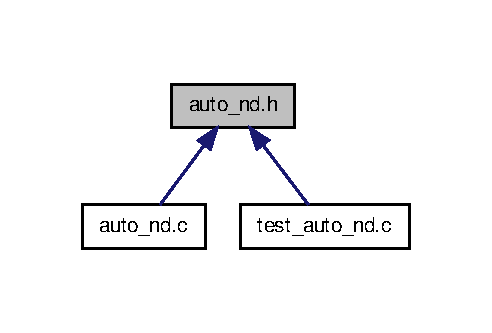
\includegraphics[width=236pt]{auto__nd_8h__dep__incl}
\end{center}
\end{figure}
\subsection*{\-Structures de données}
\begin{DoxyCompactItemize}
\item 
struct \hyperlink{struct_transition}{\-Transition}
\begin{DoxyCompactList}\small\item\em \-Objet fonction de transition. \end{DoxyCompactList}\item 
struct \hyperlink{struct_automate___n_d}{\-Automate\-\_\-\-N\-D}
\begin{DoxyCompactList}\small\item\em \-Objet automate indéterministe. \end{DoxyCompactList}\end{DoxyCompactItemize}
\subsection*{\-Macros}
\begin{DoxyCompactItemize}
\item 
\#define \hyperlink{auto__nd_8h_a01c9c2bc0eb92ea10d0d8ffe2444aa90}{\-Entier}~int
\item 
\#define \hyperlink{auto__nd_8h_a725c798f5e7ed9a07c672cb966f35ce1}{\-Char}~char
\item 
\#define \hyperlink{auto__nd_8h_a04b323d3d7ddb72161c7d0a8ba6b20b6}{\-Chaine}~char$\ast$
\item 
\#define \hyperlink{auto__nd_8h_af377ca31aa805000f5287ecb041d90df}{\-Ensemble\-Etat}~int$\ast$
\item 
\#define \hyperlink{auto__nd_8h_a8a9f3c362f156e37cdf72bfac024d7e3}{\-Ensemble\-Char}~char$\ast$
\item 
\#define \hyperlink{auto__nd_8h_abefd29f277cc57fe5d7540dcfa9c9edc}{\-Ensemble\-Transition}~\hyperlink{struct_transition}{\-Transition}$\ast$
\end{DoxyCompactItemize}
\subsection*{\-Définitions de type}
\begin{DoxyCompactItemize}
\item 
typedef \hyperlink{auto__nd_8h_a01c9c2bc0eb92ea10d0d8ffe2444aa90}{\-Entier} \hyperlink{auto__nd_8h_aae0c86cf5eb18ae170b50062873cb0c1}{\-Etat}
\item 
typedef \hyperlink{auto__nd_8h_af377ca31aa805000f5287ecb041d90df}{\-Ensemble\-Etat} \hyperlink{auto__nd_8h_ab97da0c1b1e5f14d8f0cec086e90fece}{\-Ets}
\item 
typedef struct \hyperlink{struct_transition}{\-Transition} $\ast$ \hyperlink{auto__nd_8h_a83a8cfaf050dadd5e51f6bb00d0dee6a}{\-Transition}
\item 
typedef struct \hyperlink{struct_automate___n_d}{\-Automate\-\_\-\-N\-D} $\ast$ \hyperlink{auto__nd_8h_a9fc9b66075644376db177bb7337bcb71}{\-Automate\-\_\-\-N\-D}
\end{DoxyCompactItemize}
\subsection*{\-Fonctions}
\begin{DoxyCompactItemize}
\item 
\hyperlink{struct_automate___n_d}{\-Automate\-\_\-\-N\-D} \hyperlink{auto__nd_8h_af69591ffe63ee61cfca113793e74a52a}{auto\-\_\-nd\-\_\-creer} ()
\begin{DoxyCompactList}\small\item\em \-Création d'un automate indéterministe vide. \end{DoxyCompactList}\item 
\hyperlink{struct_automate___n_d}{\-Automate\-\_\-\-N\-D} \hyperlink{auto__nd_8h_aaffcc81be17700a307595e9021d365dd}{auto\-\_\-nd\-\_\-creer\-P} (\hyperlink{auto__nd_8h_a8a9f3c362f156e37cdf72bfac024d7e3}{\-Ensemble\-Char} s, \hyperlink{auto__nd_8h_ab97da0c1b1e5f14d8f0cec086e90fece}{\-Ets} e, \hyperlink{auto__nd_8h_ab97da0c1b1e5f14d8f0cec086e90fece}{\-Ets} i, \hyperlink{auto__nd_8h_ab97da0c1b1e5f14d8f0cec086e90fece}{\-Ets} f, \hyperlink{auto__nd_8h_abefd29f277cc57fe5d7540dcfa9c9edc}{\-Ensemble\-Transition} d)
\begin{DoxyCompactList}\small\item\em \-Création d'un automate indéterministe non vide. \end{DoxyCompactList}\item 
int \hyperlink{auto__nd_8h_aa3d2073dcce65ddd666e94f4ec54436e}{auto\-\_\-nd\-\_\-detruire} (\hyperlink{struct_automate___n_d}{\-Automate\-\_\-\-N\-D} auto\-\_\-nd)
\begin{DoxyCompactList}\small\item\em \-Destruction d'un automate indéterministe. \end{DoxyCompactList}\item 
\hyperlink{struct_automate___n_d}{\-Automate\-\_\-\-N\-D} \hyperlink{auto__nd_8h_a212359ae461e94794fe0c56881505be5}{auto\-\_\-nd\-\_\-clone} (\hyperlink{struct_automate___n_d}{\-Automate\-\_\-\-N\-D} auto\-\_\-nd)
\begin{DoxyCompactList}\small\item\em \-Clonage d'un automate indéterministe. \end{DoxyCompactList}\item 
\hyperlink{auto__nd_8h_a04b323d3d7ddb72161c7d0a8ba6b20b6}{\-Chaine} \hyperlink{auto__nd_8h_a0b4c03d4ca0c54f969aa619b017294cd}{auto\-\_\-nd\-\_\-chaine} (\hyperlink{struct_automate___n_d}{\-Automate\-\_\-\-N\-D} auto\-\_\-nd)
\begin{DoxyCompactList}\small\item\em \-Description d'un automate indéterministe. \end{DoxyCompactList}\item 
int \hyperlink{auto__nd_8h_a27515409d8bce85f300634555e05e763}{auto\-\_\-nd\-\_\-appartient} (char $\ast$mot, \hyperlink{struct_automate___n_d}{\-Automate\-\_\-\-N\-D} auto\-\_\-nd)
\item 
int \hyperlink{auto__nd_8h_a79d94e6387dfdcf608f4725352d79f94}{auto\-\_\-nd\-\_\-accessible} (\hyperlink{auto__nd_8h_aae0c86cf5eb18ae170b50062873cb0c1}{\-Etat} e, \hyperlink{struct_automate___n_d}{\-Automate\-\_\-\-N\-D} auto\-\_\-nd)
\item 
int \hyperlink{auto__nd_8h_afe137460d216b118270adf740722bd27}{auto\-\_\-nd\-\_\-coaccessible} (\hyperlink{auto__nd_8h_aae0c86cf5eb18ae170b50062873cb0c1}{\-Etat} e, \hyperlink{struct_automate___n_d}{\-Automate\-\_\-\-N\-D} auto\-\_\-nd)
\item 
int \hyperlink{auto__nd_8h_a3f3692af6a52ea59d2fb11706aa0e5b3}{auto\-\_\-nd\-\_\-jumeaux} (\hyperlink{struct_automate___n_d}{\-Automate\-\_\-\-N\-D} auto\-\_\-nd1, \hyperlink{struct_automate___n_d}{\-Automate\-\_\-\-N\-D} auto\-\_\-nd2)
\item 
int \hyperlink{auto__nd_8h_a3f519dfe982a416e1817ad4baf7b6370}{auto\-\_\-nd\-\_\-equivalents} (\hyperlink{struct_automate___n_d}{\-Automate\-\_\-\-N\-D} auto\-\_\-nd1, \hyperlink{struct_automate___n_d}{\-Automate\-\_\-\-N\-D} auto\-\_\-nd2)
\item 
int \hyperlink{auto__nd_8h_a1a3c107277000a6257a89a8480ee1afd}{auto\-\_\-nd\-\_\-nb\-Lettres} (\hyperlink{struct_automate___n_d}{\-Automate\-\_\-\-N\-D} auto\-\_\-nd)
\item 
int \hyperlink{auto__nd_8h_a61fe4e60e7bc060738643fd05c8932a0}{auto\-\_\-nd\-\_\-nb\-Etats} (\hyperlink{struct_automate___n_d}{\-Automate\-\_\-\-N\-D} auto\-\_\-nd)
\item 
int \hyperlink{auto__nd_8h_a31a554bb355b78f8c9650e0ad2494619}{auto\-\_\-nd\-\_\-nb\-Initiaux} (\hyperlink{struct_automate___n_d}{\-Automate\-\_\-\-N\-D} auto\-\_\-nd)
\item 
int \hyperlink{auto__nd_8h_a6a77bca76f0c078d5c77a7d58ae1f680}{auto\-\_\-nd\-\_\-nb\-Finaux} (\hyperlink{struct_automate___n_d}{\-Automate\-\_\-\-N\-D} auto\-\_\-nd)
\item 
int \hyperlink{auto__nd_8h_a377f0d84c496692b423d7df61fa2d85a}{auto\-\_\-nd\-\_\-nb\-Transitions} (\hyperlink{struct_automate___n_d}{\-Automate\-\_\-\-N\-D} auto\-\_\-nd)
\item 
void \hyperlink{auto__nd_8h_a13d95e7cd464eef2ce273946506b96f4}{auto\-\_\-nd\-\_\-ajout\-Lettre} (char c, \hyperlink{struct_automate___n_d}{\-Automate\-\_\-\-N\-D} auto\-\_\-nd)
\item 
void \hyperlink{auto__nd_8h_a699f7374d01be804c5d5a0f2d8ee8872}{auto\-\_\-nd\-\_\-ajout\-Etat} (\hyperlink{auto__nd_8h_aae0c86cf5eb18ae170b50062873cb0c1}{\-Etat} e, \hyperlink{struct_automate___n_d}{\-Automate\-\_\-\-N\-D} auto\-\_\-nd)
\item 
void \hyperlink{auto__nd_8h_ae290407f1418df8dd0cb1a612901ae37}{auto\-\_\-nd\-\_\-ajout\-Initial} (\hyperlink{auto__nd_8h_aae0c86cf5eb18ae170b50062873cb0c1}{\-Etat} i, \hyperlink{struct_automate___n_d}{\-Automate\-\_\-\-N\-D} auto\-\_\-nd)
\item 
void \hyperlink{auto__nd_8h_ad92ce4c86d5d4f695e614eba93a90c82}{auto\-\_\-nd\-\_\-ajout\-Final} (\hyperlink{auto__nd_8h_aae0c86cf5eb18ae170b50062873cb0c1}{\-Etat} f, \hyperlink{struct_automate___n_d}{\-Automate\-\_\-\-N\-D} auto\-\_\-nd)
\item 
void \hyperlink{auto__nd_8h_ab4389b9b99010af37b0a1f55ba565a35}{auto\-\_\-nd\-\_\-ajout\-Transition} (\hyperlink{struct_transition}{\-Transition} t, \hyperlink{struct_automate___n_d}{\-Automate\-\_\-\-N\-D} auto\-\_\-nd)
\item 
void \hyperlink{auto__nd_8h_a71fd5b027c59c569247c144a97aac72f}{auto\-\_\-nd\-\_\-suppr\-Lettre} (char c, \hyperlink{struct_automate___n_d}{\-Automate\-\_\-\-N\-D} auto\-\_\-nd)
\item 
void \hyperlink{auto__nd_8h_abc8e956fda2f30bc3af985a4a002a5ee}{auto\-\_\-nd\-\_\-suppr\-Etat} (\hyperlink{auto__nd_8h_aae0c86cf5eb18ae170b50062873cb0c1}{\-Etat} e, \hyperlink{struct_automate___n_d}{\-Automate\-\_\-\-N\-D} auto\-\_\-nd)
\item 
void \hyperlink{auto__nd_8h_aca2642240007ce7acab36a6ddc994a69}{auto\-\_\-nd\-\_\-suppr\-Transition} (\hyperlink{struct_transition}{\-Transition} t, \hyperlink{struct_automate___n_d}{\-Automate\-\_\-\-N\-D} auto\-\_\-nd)
\item 
\hyperlink{struct_automate___n_d}{\-Automate\-\_\-\-N\-D} \hyperlink{auto__nd_8h_a5bd71be0cb8a4c522c1ee818496983c5}{auto\-\_\-nd\-\_\-completer} (\hyperlink{struct_automate___n_d}{\-Automate\-\_\-\-N\-D} auto\-\_\-nd)
\item 
\hyperlink{struct_automate___n_d}{\-Automate\-\_\-\-N\-D} \hyperlink{auto__nd_8h_a2649a06ebe3a71986c20371c16465636}{auto\-\_\-nd\-\_\-reduire} (\hyperlink{struct_automate___n_d}{\-Automate\-\_\-\-N\-D} auto\-\_\-nd)
\item 
\hyperlink{auto__nd_8h_a04b323d3d7ddb72161c7d0a8ba6b20b6}{\-Chaine} \hyperlink{auto__nd_8h_a956166e9403f28b1544dbc475db7afee}{auto\-\_\-nd\-\_\-liste\-Mots} (int debut, int fin, \hyperlink{struct_automate___n_d}{\-Automate\-\_\-\-N\-D} auto\-\_\-nd)
\item 
\hyperlink{auto__nd_8h_a04b323d3d7ddb72161c7d0a8ba6b20b6}{\-Chaine} \hyperlink{auto__nd_8h_aa18a4077a0868825391d5737fa0c8d29}{auto\-\_\-nd\-\_\-liste\-Mots\-Alpha} (int debut, int fin, \hyperlink{struct_automate___n_d}{\-Automate\-\_\-\-N\-D} auto\-\_\-nd)
\item 
\hyperlink{auto__nd_8h_a04b323d3d7ddb72161c7d0a8ba6b20b6}{\-Chaine} \hyperlink{auto__nd_8h_a269f375009f4853e3f08f38142dbb2e2}{auto\-\_\-nd\-\_\-chemin} (char $\ast$mot, \hyperlink{struct_automate___n_d}{\-Automate\-\_\-\-N\-D} auto\-\_\-nd)
\item 
\hyperlink{auto__nd_8h_a04b323d3d7ddb72161c7d0a8ba6b20b6}{\-Chaine} \hyperlink{auto__nd_8h_a8b25b03f74ee27486bbe15f29c9d5aa7}{auto\-\_\-nd\-\_\-chemins} (char $\ast$mot, \hyperlink{struct_automate___n_d}{\-Automate\-\_\-\-N\-D} auto\-\_\-nd)
\item 
int \hyperlink{auto__nd_8h_ad2d27eb4a14392cbb539d56d41524318}{auto\-\_\-nd\-\_\-nb\-Chemins\-Possibles} (char $\ast$mot, \hyperlink{struct_automate___n_d}{\-Automate\-\_\-\-N\-D} auto\-\_\-nd)
\end{DoxyCompactItemize}


\subsection{\-Description détaillée}
\-Header des \-Automates indéterministes. \begin{DoxyAuthor}{\-Auteur}
\-Gauthier \-Silvère
\end{DoxyAuthor}
\-Fichier de définition des types, structures et fonctions concernant les automates indéterministes. 

\-Définition dans le fichier \hyperlink{auto__nd_8h_source}{auto\-\_\-nd.\-h}.



\subsection{\-Documentation des macros}
\hypertarget{auto__nd_8h_a04b323d3d7ddb72161c7d0a8ba6b20b6}{\index{auto\-\_\-nd.\-h@{auto\-\_\-nd.\-h}!\-Chaine@{\-Chaine}}
\index{\-Chaine@{\-Chaine}!auto_nd.h@{auto\-\_\-nd.\-h}}
\subsubsection[{\-Chaine}]{\setlength{\rightskip}{0pt plus 5cm}\#define {\bf \-Chaine}~char$\ast$}}\label{auto__nd_8h_a04b323d3d7ddb72161c7d0a8ba6b20b6}


\-Définition à la ligne 15 du fichier auto\-\_\-nd.\-h.

\hypertarget{auto__nd_8h_a725c798f5e7ed9a07c672cb966f35ce1}{\index{auto\-\_\-nd.\-h@{auto\-\_\-nd.\-h}!\-Char@{\-Char}}
\index{\-Char@{\-Char}!auto_nd.h@{auto\-\_\-nd.\-h}}
\subsubsection[{\-Char}]{\setlength{\rightskip}{0pt plus 5cm}\#define {\bf \-Char}~char}}\label{auto__nd_8h_a725c798f5e7ed9a07c672cb966f35ce1}


\-Définition à la ligne 14 du fichier auto\-\_\-nd.\-h.

\hypertarget{auto__nd_8h_a8a9f3c362f156e37cdf72bfac024d7e3}{\index{auto\-\_\-nd.\-h@{auto\-\_\-nd.\-h}!\-Ensemble\-Char@{\-Ensemble\-Char}}
\index{\-Ensemble\-Char@{\-Ensemble\-Char}!auto_nd.h@{auto\-\_\-nd.\-h}}
\subsubsection[{\-Ensemble\-Char}]{\setlength{\rightskip}{0pt plus 5cm}\#define {\bf \-Ensemble\-Char}~char$\ast$}}\label{auto__nd_8h_a8a9f3c362f156e37cdf72bfac024d7e3}


\-Définition à la ligne 17 du fichier auto\-\_\-nd.\-h.

\hypertarget{auto__nd_8h_af377ca31aa805000f5287ecb041d90df}{\index{auto\-\_\-nd.\-h@{auto\-\_\-nd.\-h}!\-Ensemble\-Etat@{\-Ensemble\-Etat}}
\index{\-Ensemble\-Etat@{\-Ensemble\-Etat}!auto_nd.h@{auto\-\_\-nd.\-h}}
\subsubsection[{\-Ensemble\-Etat}]{\setlength{\rightskip}{0pt plus 5cm}\#define {\bf \-Ensemble\-Etat}~int$\ast$}}\label{auto__nd_8h_af377ca31aa805000f5287ecb041d90df}


\-Définition à la ligne 16 du fichier auto\-\_\-nd.\-h.

\hypertarget{auto__nd_8h_abefd29f277cc57fe5d7540dcfa9c9edc}{\index{auto\-\_\-nd.\-h@{auto\-\_\-nd.\-h}!\-Ensemble\-Transition@{\-Ensemble\-Transition}}
\index{\-Ensemble\-Transition@{\-Ensemble\-Transition}!auto_nd.h@{auto\-\_\-nd.\-h}}
\subsubsection[{\-Ensemble\-Transition}]{\setlength{\rightskip}{0pt plus 5cm}\#define {\bf \-Ensemble\-Transition}~{\bf \-Transition}$\ast$}}\label{auto__nd_8h_abefd29f277cc57fe5d7540dcfa9c9edc}


\-Définition à la ligne 18 du fichier auto\-\_\-nd.\-h.

\hypertarget{auto__nd_8h_a01c9c2bc0eb92ea10d0d8ffe2444aa90}{\index{auto\-\_\-nd.\-h@{auto\-\_\-nd.\-h}!\-Entier@{\-Entier}}
\index{\-Entier@{\-Entier}!auto_nd.h@{auto\-\_\-nd.\-h}}
\subsubsection[{\-Entier}]{\setlength{\rightskip}{0pt plus 5cm}\#define {\bf \-Entier}~int}}\label{auto__nd_8h_a01c9c2bc0eb92ea10d0d8ffe2444aa90}


\-Définition à la ligne 13 du fichier auto\-\_\-nd.\-h.



\subsection{\-Documentation des définitions de type}
\hypertarget{auto__nd_8h_a9fc9b66075644376db177bb7337bcb71}{\index{auto\-\_\-nd.\-h@{auto\-\_\-nd.\-h}!\-Automate\-\_\-\-N\-D@{\-Automate\-\_\-\-N\-D}}
\index{\-Automate\-\_\-\-N\-D@{\-Automate\-\_\-\-N\-D}!auto_nd.h@{auto\-\_\-nd.\-h}}
\subsubsection[{\-Automate\-\_\-\-N\-D}]{\setlength{\rightskip}{0pt plus 5cm}typedef struct {\bf \-Automate\-\_\-\-N\-D} $\ast$ {\bf \-Automate\-\_\-\-N\-D}}}\label{auto__nd_8h_a9fc9b66075644376db177bb7337bcb71}
\hypertarget{auto__nd_8h_aae0c86cf5eb18ae170b50062873cb0c1}{\index{auto\-\_\-nd.\-h@{auto\-\_\-nd.\-h}!\-Etat@{\-Etat}}
\index{\-Etat@{\-Etat}!auto_nd.h@{auto\-\_\-nd.\-h}}
\subsubsection[{\-Etat}]{\setlength{\rightskip}{0pt plus 5cm}typedef {\bf \-Entier} {\bf \-Etat}}}\label{auto__nd_8h_aae0c86cf5eb18ae170b50062873cb0c1}
\-Types abstraits utilisés pour les automates indéterministes. 

\-Définition à la ligne 28 du fichier auto\-\_\-nd.\-h.

\hypertarget{auto__nd_8h_ab97da0c1b1e5f14d8f0cec086e90fece}{\index{auto\-\_\-nd.\-h@{auto\-\_\-nd.\-h}!\-Ets@{\-Ets}}
\index{\-Ets@{\-Ets}!auto_nd.h@{auto\-\_\-nd.\-h}}
\subsubsection[{\-Ets}]{\setlength{\rightskip}{0pt plus 5cm}typedef {\bf \-Ensemble\-Etat} {\bf \-Ets}}}\label{auto__nd_8h_ab97da0c1b1e5f14d8f0cec086e90fece}


\-Définition à la ligne 29 du fichier auto\-\_\-nd.\-h.

\hypertarget{auto__nd_8h_a83a8cfaf050dadd5e51f6bb00d0dee6a}{\index{auto\-\_\-nd.\-h@{auto\-\_\-nd.\-h}!\-Transition@{\-Transition}}
\index{\-Transition@{\-Transition}!auto_nd.h@{auto\-\_\-nd.\-h}}
\subsubsection[{\-Transition}]{\setlength{\rightskip}{0pt plus 5cm}typedef struct {\bf \-Transition}$\ast$  {\bf \-Transition}}}\label{auto__nd_8h_a83a8cfaf050dadd5e51f6bb00d0dee6a}


\subsection{\-Documentation des fonctions}
\hypertarget{auto__nd_8h_a79d94e6387dfdcf608f4725352d79f94}{\index{auto\-\_\-nd.\-h@{auto\-\_\-nd.\-h}!auto\-\_\-nd\-\_\-accessible@{auto\-\_\-nd\-\_\-accessible}}
\index{auto\-\_\-nd\-\_\-accessible@{auto\-\_\-nd\-\_\-accessible}!auto_nd.h@{auto\-\_\-nd.\-h}}
\subsubsection[{auto\-\_\-nd\-\_\-accessible}]{\setlength{\rightskip}{0pt plus 5cm}int {\bf auto\-\_\-nd\-\_\-accessible} (
\begin{DoxyParamCaption}
\item[{{\bf \-Etat}}]{e, }
\item[{{\bf \-Automate\-\_\-\-N\-D}}]{auto\-\_\-nd}
\end{DoxyParamCaption}
)}}\label{auto__nd_8h_a79d94e6387dfdcf608f4725352d79f94}
\hypertarget{auto__nd_8h_a699f7374d01be804c5d5a0f2d8ee8872}{\index{auto\-\_\-nd.\-h@{auto\-\_\-nd.\-h}!auto\-\_\-nd\-\_\-ajout\-Etat@{auto\-\_\-nd\-\_\-ajout\-Etat}}
\index{auto\-\_\-nd\-\_\-ajout\-Etat@{auto\-\_\-nd\-\_\-ajout\-Etat}!auto_nd.h@{auto\-\_\-nd.\-h}}
\subsubsection[{auto\-\_\-nd\-\_\-ajout\-Etat}]{\setlength{\rightskip}{0pt plus 5cm}void {\bf auto\-\_\-nd\-\_\-ajout\-Etat} (
\begin{DoxyParamCaption}
\item[{{\bf \-Etat}}]{e, }
\item[{{\bf \-Automate\-\_\-\-N\-D}}]{auto\-\_\-nd}
\end{DoxyParamCaption}
)}}\label{auto__nd_8h_a699f7374d01be804c5d5a0f2d8ee8872}
\hypertarget{auto__nd_8h_ad92ce4c86d5d4f695e614eba93a90c82}{\index{auto\-\_\-nd.\-h@{auto\-\_\-nd.\-h}!auto\-\_\-nd\-\_\-ajout\-Final@{auto\-\_\-nd\-\_\-ajout\-Final}}
\index{auto\-\_\-nd\-\_\-ajout\-Final@{auto\-\_\-nd\-\_\-ajout\-Final}!auto_nd.h@{auto\-\_\-nd.\-h}}
\subsubsection[{auto\-\_\-nd\-\_\-ajout\-Final}]{\setlength{\rightskip}{0pt plus 5cm}void {\bf auto\-\_\-nd\-\_\-ajout\-Final} (
\begin{DoxyParamCaption}
\item[{{\bf \-Etat}}]{f, }
\item[{{\bf \-Automate\-\_\-\-N\-D}}]{auto\-\_\-nd}
\end{DoxyParamCaption}
)}}\label{auto__nd_8h_ad92ce4c86d5d4f695e614eba93a90c82}
\hypertarget{auto__nd_8h_ae290407f1418df8dd0cb1a612901ae37}{\index{auto\-\_\-nd.\-h@{auto\-\_\-nd.\-h}!auto\-\_\-nd\-\_\-ajout\-Initial@{auto\-\_\-nd\-\_\-ajout\-Initial}}
\index{auto\-\_\-nd\-\_\-ajout\-Initial@{auto\-\_\-nd\-\_\-ajout\-Initial}!auto_nd.h@{auto\-\_\-nd.\-h}}
\subsubsection[{auto\-\_\-nd\-\_\-ajout\-Initial}]{\setlength{\rightskip}{0pt plus 5cm}void {\bf auto\-\_\-nd\-\_\-ajout\-Initial} (
\begin{DoxyParamCaption}
\item[{{\bf \-Etat}}]{i, }
\item[{{\bf \-Automate\-\_\-\-N\-D}}]{auto\-\_\-nd}
\end{DoxyParamCaption}
)}}\label{auto__nd_8h_ae290407f1418df8dd0cb1a612901ae37}
\hypertarget{auto__nd_8h_a13d95e7cd464eef2ce273946506b96f4}{\index{auto\-\_\-nd.\-h@{auto\-\_\-nd.\-h}!auto\-\_\-nd\-\_\-ajout\-Lettre@{auto\-\_\-nd\-\_\-ajout\-Lettre}}
\index{auto\-\_\-nd\-\_\-ajout\-Lettre@{auto\-\_\-nd\-\_\-ajout\-Lettre}!auto_nd.h@{auto\-\_\-nd.\-h}}
\subsubsection[{auto\-\_\-nd\-\_\-ajout\-Lettre}]{\setlength{\rightskip}{0pt plus 5cm}void {\bf auto\-\_\-nd\-\_\-ajout\-Lettre} (
\begin{DoxyParamCaption}
\item[{char}]{c, }
\item[{{\bf \-Automate\-\_\-\-N\-D}}]{auto\-\_\-nd}
\end{DoxyParamCaption}
)}}\label{auto__nd_8h_a13d95e7cd464eef2ce273946506b96f4}
\hypertarget{auto__nd_8h_ab4389b9b99010af37b0a1f55ba565a35}{\index{auto\-\_\-nd.\-h@{auto\-\_\-nd.\-h}!auto\-\_\-nd\-\_\-ajout\-Transition@{auto\-\_\-nd\-\_\-ajout\-Transition}}
\index{auto\-\_\-nd\-\_\-ajout\-Transition@{auto\-\_\-nd\-\_\-ajout\-Transition}!auto_nd.h@{auto\-\_\-nd.\-h}}
\subsubsection[{auto\-\_\-nd\-\_\-ajout\-Transition}]{\setlength{\rightskip}{0pt plus 5cm}void {\bf auto\-\_\-nd\-\_\-ajout\-Transition} (
\begin{DoxyParamCaption}
\item[{{\bf \-Transition}}]{t, }
\item[{{\bf \-Automate\-\_\-\-N\-D}}]{auto\-\_\-nd}
\end{DoxyParamCaption}
)}}\label{auto__nd_8h_ab4389b9b99010af37b0a1f55ba565a35}
\hypertarget{auto__nd_8h_a27515409d8bce85f300634555e05e763}{\index{auto\-\_\-nd.\-h@{auto\-\_\-nd.\-h}!auto\-\_\-nd\-\_\-appartient@{auto\-\_\-nd\-\_\-appartient}}
\index{auto\-\_\-nd\-\_\-appartient@{auto\-\_\-nd\-\_\-appartient}!auto_nd.h@{auto\-\_\-nd.\-h}}
\subsubsection[{auto\-\_\-nd\-\_\-appartient}]{\setlength{\rightskip}{0pt plus 5cm}int {\bf auto\-\_\-nd\-\_\-appartient} (
\begin{DoxyParamCaption}
\item[{char $\ast$}]{mot, }
\item[{{\bf \-Automate\-\_\-\-N\-D}}]{auto\-\_\-nd}
\end{DoxyParamCaption}
)}}\label{auto__nd_8h_a27515409d8bce85f300634555e05e763}
\hypertarget{auto__nd_8h_a0b4c03d4ca0c54f969aa619b017294cd}{\index{auto\-\_\-nd.\-h@{auto\-\_\-nd.\-h}!auto\-\_\-nd\-\_\-chaine@{auto\-\_\-nd\-\_\-chaine}}
\index{auto\-\_\-nd\-\_\-chaine@{auto\-\_\-nd\-\_\-chaine}!auto_nd.h@{auto\-\_\-nd.\-h}}
\subsubsection[{auto\-\_\-nd\-\_\-chaine}]{\setlength{\rightskip}{0pt plus 5cm}{\bf \-Chaine} {\bf auto\-\_\-nd\-\_\-chaine} (
\begin{DoxyParamCaption}
\item[{{\bf \-Automate\-\_\-\-N\-D}}]{auto\-\_\-nd}
\end{DoxyParamCaption}
)}}\label{auto__nd_8h_a0b4c03d4ca0c54f969aa619b017294cd}


\-Description d'un automate indéterministe. 


\begin{DoxyParams}[1]{\-Paramètres}
\mbox{\tt in}  & {\em auto\-\_\-nd} & \-Automate à décrire. \\
\hline
\end{DoxyParams}
\begin{DoxyReturn}{\-Renvoie}
\-Chaîne de caractères décrivant l'automate indéterministe passé en paramètre. 
\end{DoxyReturn}


\-Définition à la ligne 50 du fichier auto\-\_\-nd.\-c.

\hypertarget{auto__nd_8h_a269f375009f4853e3f08f38142dbb2e2}{\index{auto\-\_\-nd.\-h@{auto\-\_\-nd.\-h}!auto\-\_\-nd\-\_\-chemin@{auto\-\_\-nd\-\_\-chemin}}
\index{auto\-\_\-nd\-\_\-chemin@{auto\-\_\-nd\-\_\-chemin}!auto_nd.h@{auto\-\_\-nd.\-h}}
\subsubsection[{auto\-\_\-nd\-\_\-chemin}]{\setlength{\rightskip}{0pt plus 5cm}{\bf \-Chaine} {\bf auto\-\_\-nd\-\_\-chemin} (
\begin{DoxyParamCaption}
\item[{char $\ast$}]{mot, }
\item[{{\bf \-Automate\-\_\-\-N\-D}}]{auto\-\_\-nd}
\end{DoxyParamCaption}
)}}\label{auto__nd_8h_a269f375009f4853e3f08f38142dbb2e2}
\hypertarget{auto__nd_8h_a8b25b03f74ee27486bbe15f29c9d5aa7}{\index{auto\-\_\-nd.\-h@{auto\-\_\-nd.\-h}!auto\-\_\-nd\-\_\-chemins@{auto\-\_\-nd\-\_\-chemins}}
\index{auto\-\_\-nd\-\_\-chemins@{auto\-\_\-nd\-\_\-chemins}!auto_nd.h@{auto\-\_\-nd.\-h}}
\subsubsection[{auto\-\_\-nd\-\_\-chemins}]{\setlength{\rightskip}{0pt plus 5cm}{\bf \-Chaine} {\bf auto\-\_\-nd\-\_\-chemins} (
\begin{DoxyParamCaption}
\item[{char $\ast$}]{mot, }
\item[{{\bf \-Automate\-\_\-\-N\-D}}]{auto\-\_\-nd}
\end{DoxyParamCaption}
)}}\label{auto__nd_8h_a8b25b03f74ee27486bbe15f29c9d5aa7}
\hypertarget{auto__nd_8h_a212359ae461e94794fe0c56881505be5}{\index{auto\-\_\-nd.\-h@{auto\-\_\-nd.\-h}!auto\-\_\-nd\-\_\-clone@{auto\-\_\-nd\-\_\-clone}}
\index{auto\-\_\-nd\-\_\-clone@{auto\-\_\-nd\-\_\-clone}!auto_nd.h@{auto\-\_\-nd.\-h}}
\subsubsection[{auto\-\_\-nd\-\_\-clone}]{\setlength{\rightskip}{0pt plus 5cm}{\bf \-Automate\-\_\-\-N\-D} {\bf auto\-\_\-nd\-\_\-clone} (
\begin{DoxyParamCaption}
\item[{{\bf \-Automate\-\_\-\-N\-D}}]{auto\-\_\-nd}
\end{DoxyParamCaption}
)}}\label{auto__nd_8h_a212359ae461e94794fe0c56881505be5}


\-Clonage d'un automate indéterministe. 


\begin{DoxyParams}[1]{\-Paramètres}
\mbox{\tt in}  & {\em auto\-\_\-nd} & \-Automate à cloner. \\
\hline
\end{DoxyParams}
\begin{DoxyReturn}{\-Renvoie}
\-Instance nouvelle d'un \hyperlink{struct_automate___n_d}{\-Automate\-\_\-\-N\-D} alloué d'ensembles identiques à auto\-\_\-nd (par copie). 
\end{DoxyReturn}


\-Définition à la ligne 46 du fichier auto\-\_\-nd.\-c.

\hypertarget{auto__nd_8h_afe137460d216b118270adf740722bd27}{\index{auto\-\_\-nd.\-h@{auto\-\_\-nd.\-h}!auto\-\_\-nd\-\_\-coaccessible@{auto\-\_\-nd\-\_\-coaccessible}}
\index{auto\-\_\-nd\-\_\-coaccessible@{auto\-\_\-nd\-\_\-coaccessible}!auto_nd.h@{auto\-\_\-nd.\-h}}
\subsubsection[{auto\-\_\-nd\-\_\-coaccessible}]{\setlength{\rightskip}{0pt plus 5cm}int {\bf auto\-\_\-nd\-\_\-coaccessible} (
\begin{DoxyParamCaption}
\item[{{\bf \-Etat}}]{e, }
\item[{{\bf \-Automate\-\_\-\-N\-D}}]{auto\-\_\-nd}
\end{DoxyParamCaption}
)}}\label{auto__nd_8h_afe137460d216b118270adf740722bd27}
\hypertarget{auto__nd_8h_a5bd71be0cb8a4c522c1ee818496983c5}{\index{auto\-\_\-nd.\-h@{auto\-\_\-nd.\-h}!auto\-\_\-nd\-\_\-completer@{auto\-\_\-nd\-\_\-completer}}
\index{auto\-\_\-nd\-\_\-completer@{auto\-\_\-nd\-\_\-completer}!auto_nd.h@{auto\-\_\-nd.\-h}}
\subsubsection[{auto\-\_\-nd\-\_\-completer}]{\setlength{\rightskip}{0pt plus 5cm}{\bf \-Automate\-\_\-\-N\-D} {\bf auto\-\_\-nd\-\_\-completer} (
\begin{DoxyParamCaption}
\item[{{\bf \-Automate\-\_\-\-N\-D}}]{auto\-\_\-nd}
\end{DoxyParamCaption}
)}}\label{auto__nd_8h_a5bd71be0cb8a4c522c1ee818496983c5}
\hypertarget{auto__nd_8h_af69591ffe63ee61cfca113793e74a52a}{\index{auto\-\_\-nd.\-h@{auto\-\_\-nd.\-h}!auto\-\_\-nd\-\_\-creer@{auto\-\_\-nd\-\_\-creer}}
\index{auto\-\_\-nd\-\_\-creer@{auto\-\_\-nd\-\_\-creer}!auto_nd.h@{auto\-\_\-nd.\-h}}
\subsubsection[{auto\-\_\-nd\-\_\-creer}]{\setlength{\rightskip}{0pt plus 5cm}{\bf \-Automate\-\_\-\-N\-D} {\bf auto\-\_\-nd\-\_\-creer} (
\begin{DoxyParamCaption}
{}
\end{DoxyParamCaption}
)}}\label{auto__nd_8h_af69591ffe63ee61cfca113793e74a52a}


\-Création d'un automate indéterministe vide. 

\begin{DoxyReturn}{\-Renvoie}
\-Instance nouvelle d'un \hyperlink{struct_automate___n_d}{\-Automate\-\_\-\-N\-D} alloué d'ensembles vides. 
\end{DoxyReturn}


\-Définition à la ligne 18 du fichier auto\-\_\-nd.\-c.

\hypertarget{auto__nd_8h_aaffcc81be17700a307595e9021d365dd}{\index{auto\-\_\-nd.\-h@{auto\-\_\-nd.\-h}!auto\-\_\-nd\-\_\-creer\-P@{auto\-\_\-nd\-\_\-creer\-P}}
\index{auto\-\_\-nd\-\_\-creer\-P@{auto\-\_\-nd\-\_\-creer\-P}!auto_nd.h@{auto\-\_\-nd.\-h}}
\subsubsection[{auto\-\_\-nd\-\_\-creer\-P}]{\setlength{\rightskip}{0pt plus 5cm}{\bf \-Automate\-\_\-\-N\-D} {\bf auto\-\_\-nd\-\_\-creer\-P} (
\begin{DoxyParamCaption}
\item[{{\bf \-Ensemble\-Char}}]{s, }
\item[{{\bf \-Ets}}]{e, }
\item[{{\bf \-Ets}}]{i, }
\item[{{\bf \-Ets}}]{f, }
\item[{{\bf \-Ensemble\-Transition}}]{d}
\end{DoxyParamCaption}
)}}\label{auto__nd_8h_aaffcc81be17700a307595e9021d365dd}


\-Création d'un automate indéterministe non vide. 


\begin{DoxyParams}[1]{\-Paramètres}
\mbox{\tt in}  & {\em s} & \-Alphabet sigma. \-Peux être vide. \\
\hline
\mbox{\tt in}  & {\em e} & \-Ensemble total d'états \-E. \-Peux être vide. \\
\hline
\mbox{\tt in}  & {\em i} & pour \-I. \-Peux être vide. \\
\hline
\mbox{\tt in}  & {\em f} & pour \-F. \-Peux être vide. \\
\hline
\mbox{\tt in}  & {\em d} & pour delta. \-Peux être vide. \\
\hline
\end{DoxyParams}
\begin{DoxyReturn}{\-Renvoie}
\-Instance nouvelle d'un \hyperlink{struct_automate___n_d}{\-Automate\-\_\-\-N\-D} alloué des ensembles passés en paramètres. 
\end{DoxyReturn}


\-Définition à la ligne 28 du fichier auto\-\_\-nd.\-c.

\hypertarget{auto__nd_8h_aa3d2073dcce65ddd666e94f4ec54436e}{\index{auto\-\_\-nd.\-h@{auto\-\_\-nd.\-h}!auto\-\_\-nd\-\_\-detruire@{auto\-\_\-nd\-\_\-detruire}}
\index{auto\-\_\-nd\-\_\-detruire@{auto\-\_\-nd\-\_\-detruire}!auto_nd.h@{auto\-\_\-nd.\-h}}
\subsubsection[{auto\-\_\-nd\-\_\-detruire}]{\setlength{\rightskip}{0pt plus 5cm}int {\bf auto\-\_\-nd\-\_\-detruire} (
\begin{DoxyParamCaption}
\item[{{\bf \-Automate\-\_\-\-N\-D}}]{auto\-\_\-nd}
\end{DoxyParamCaption}
)}}\label{auto__nd_8h_aa3d2073dcce65ddd666e94f4ec54436e}


\-Destruction d'un automate indéterministe. 


\begin{DoxyParams}[1]{\-Paramètres}
\mbox{\tt in,out}  & {\em auto\-\_\-nd} & \-Automate à détruire. \\
\hline
\end{DoxyParams}
\begin{DoxyReturn}{\-Renvoie}
0 si aucune erreur, 1 sinon. 
\end{DoxyReturn}


\-Définition à la ligne 38 du fichier auto\-\_\-nd.\-c.

\hypertarget{auto__nd_8h_a3f519dfe982a416e1817ad4baf7b6370}{\index{auto\-\_\-nd.\-h@{auto\-\_\-nd.\-h}!auto\-\_\-nd\-\_\-equivalents@{auto\-\_\-nd\-\_\-equivalents}}
\index{auto\-\_\-nd\-\_\-equivalents@{auto\-\_\-nd\-\_\-equivalents}!auto_nd.h@{auto\-\_\-nd.\-h}}
\subsubsection[{auto\-\_\-nd\-\_\-equivalents}]{\setlength{\rightskip}{0pt plus 5cm}int {\bf auto\-\_\-nd\-\_\-equivalents} (
\begin{DoxyParamCaption}
\item[{{\bf \-Automate\-\_\-\-N\-D}}]{auto\-\_\-nd1, }
\item[{{\bf \-Automate\-\_\-\-N\-D}}]{auto\-\_\-nd2}
\end{DoxyParamCaption}
)}}\label{auto__nd_8h_a3f519dfe982a416e1817ad4baf7b6370}
\hypertarget{auto__nd_8h_a3f3692af6a52ea59d2fb11706aa0e5b3}{\index{auto\-\_\-nd.\-h@{auto\-\_\-nd.\-h}!auto\-\_\-nd\-\_\-jumeaux@{auto\-\_\-nd\-\_\-jumeaux}}
\index{auto\-\_\-nd\-\_\-jumeaux@{auto\-\_\-nd\-\_\-jumeaux}!auto_nd.h@{auto\-\_\-nd.\-h}}
\subsubsection[{auto\-\_\-nd\-\_\-jumeaux}]{\setlength{\rightskip}{0pt plus 5cm}int {\bf auto\-\_\-nd\-\_\-jumeaux} (
\begin{DoxyParamCaption}
\item[{{\bf \-Automate\-\_\-\-N\-D}}]{auto\-\_\-nd1, }
\item[{{\bf \-Automate\-\_\-\-N\-D}}]{auto\-\_\-nd2}
\end{DoxyParamCaption}
)}}\label{auto__nd_8h_a3f3692af6a52ea59d2fb11706aa0e5b3}
\hypertarget{auto__nd_8h_a956166e9403f28b1544dbc475db7afee}{\index{auto\-\_\-nd.\-h@{auto\-\_\-nd.\-h}!auto\-\_\-nd\-\_\-liste\-Mots@{auto\-\_\-nd\-\_\-liste\-Mots}}
\index{auto\-\_\-nd\-\_\-liste\-Mots@{auto\-\_\-nd\-\_\-liste\-Mots}!auto_nd.h@{auto\-\_\-nd.\-h}}
\subsubsection[{auto\-\_\-nd\-\_\-liste\-Mots}]{\setlength{\rightskip}{0pt plus 5cm}{\bf \-Chaine} {\bf auto\-\_\-nd\-\_\-liste\-Mots} (
\begin{DoxyParamCaption}
\item[{int}]{debut, }
\item[{int}]{fin, }
\item[{{\bf \-Automate\-\_\-\-N\-D}}]{auto\-\_\-nd}
\end{DoxyParamCaption}
)}}\label{auto__nd_8h_a956166e9403f28b1544dbc475db7afee}
\hypertarget{auto__nd_8h_aa18a4077a0868825391d5737fa0c8d29}{\index{auto\-\_\-nd.\-h@{auto\-\_\-nd.\-h}!auto\-\_\-nd\-\_\-liste\-Mots\-Alpha@{auto\-\_\-nd\-\_\-liste\-Mots\-Alpha}}
\index{auto\-\_\-nd\-\_\-liste\-Mots\-Alpha@{auto\-\_\-nd\-\_\-liste\-Mots\-Alpha}!auto_nd.h@{auto\-\_\-nd.\-h}}
\subsubsection[{auto\-\_\-nd\-\_\-liste\-Mots\-Alpha}]{\setlength{\rightskip}{0pt plus 5cm}{\bf \-Chaine} {\bf auto\-\_\-nd\-\_\-liste\-Mots\-Alpha} (
\begin{DoxyParamCaption}
\item[{int}]{debut, }
\item[{int}]{fin, }
\item[{{\bf \-Automate\-\_\-\-N\-D}}]{auto\-\_\-nd}
\end{DoxyParamCaption}
)}}\label{auto__nd_8h_aa18a4077a0868825391d5737fa0c8d29}
\hypertarget{auto__nd_8h_ad2d27eb4a14392cbb539d56d41524318}{\index{auto\-\_\-nd.\-h@{auto\-\_\-nd.\-h}!auto\-\_\-nd\-\_\-nb\-Chemins\-Possibles@{auto\-\_\-nd\-\_\-nb\-Chemins\-Possibles}}
\index{auto\-\_\-nd\-\_\-nb\-Chemins\-Possibles@{auto\-\_\-nd\-\_\-nb\-Chemins\-Possibles}!auto_nd.h@{auto\-\_\-nd.\-h}}
\subsubsection[{auto\-\_\-nd\-\_\-nb\-Chemins\-Possibles}]{\setlength{\rightskip}{0pt plus 5cm}int {\bf auto\-\_\-nd\-\_\-nb\-Chemins\-Possibles} (
\begin{DoxyParamCaption}
\item[{char $\ast$}]{mot, }
\item[{{\bf \-Automate\-\_\-\-N\-D}}]{auto\-\_\-nd}
\end{DoxyParamCaption}
)}}\label{auto__nd_8h_ad2d27eb4a14392cbb539d56d41524318}
\hypertarget{auto__nd_8h_a61fe4e60e7bc060738643fd05c8932a0}{\index{auto\-\_\-nd.\-h@{auto\-\_\-nd.\-h}!auto\-\_\-nd\-\_\-nb\-Etats@{auto\-\_\-nd\-\_\-nb\-Etats}}
\index{auto\-\_\-nd\-\_\-nb\-Etats@{auto\-\_\-nd\-\_\-nb\-Etats}!auto_nd.h@{auto\-\_\-nd.\-h}}
\subsubsection[{auto\-\_\-nd\-\_\-nb\-Etats}]{\setlength{\rightskip}{0pt plus 5cm}int {\bf auto\-\_\-nd\-\_\-nb\-Etats} (
\begin{DoxyParamCaption}
\item[{{\bf \-Automate\-\_\-\-N\-D}}]{auto\-\_\-nd}
\end{DoxyParamCaption}
)}}\label{auto__nd_8h_a61fe4e60e7bc060738643fd05c8932a0}
\hypertarget{auto__nd_8h_a6a77bca76f0c078d5c77a7d58ae1f680}{\index{auto\-\_\-nd.\-h@{auto\-\_\-nd.\-h}!auto\-\_\-nd\-\_\-nb\-Finaux@{auto\-\_\-nd\-\_\-nb\-Finaux}}
\index{auto\-\_\-nd\-\_\-nb\-Finaux@{auto\-\_\-nd\-\_\-nb\-Finaux}!auto_nd.h@{auto\-\_\-nd.\-h}}
\subsubsection[{auto\-\_\-nd\-\_\-nb\-Finaux}]{\setlength{\rightskip}{0pt plus 5cm}int {\bf auto\-\_\-nd\-\_\-nb\-Finaux} (
\begin{DoxyParamCaption}
\item[{{\bf \-Automate\-\_\-\-N\-D}}]{auto\-\_\-nd}
\end{DoxyParamCaption}
)}}\label{auto__nd_8h_a6a77bca76f0c078d5c77a7d58ae1f680}
\hypertarget{auto__nd_8h_a31a554bb355b78f8c9650e0ad2494619}{\index{auto\-\_\-nd.\-h@{auto\-\_\-nd.\-h}!auto\-\_\-nd\-\_\-nb\-Initiaux@{auto\-\_\-nd\-\_\-nb\-Initiaux}}
\index{auto\-\_\-nd\-\_\-nb\-Initiaux@{auto\-\_\-nd\-\_\-nb\-Initiaux}!auto_nd.h@{auto\-\_\-nd.\-h}}
\subsubsection[{auto\-\_\-nd\-\_\-nb\-Initiaux}]{\setlength{\rightskip}{0pt plus 5cm}int {\bf auto\-\_\-nd\-\_\-nb\-Initiaux} (
\begin{DoxyParamCaption}
\item[{{\bf \-Automate\-\_\-\-N\-D}}]{auto\-\_\-nd}
\end{DoxyParamCaption}
)}}\label{auto__nd_8h_a31a554bb355b78f8c9650e0ad2494619}
\hypertarget{auto__nd_8h_a1a3c107277000a6257a89a8480ee1afd}{\index{auto\-\_\-nd.\-h@{auto\-\_\-nd.\-h}!auto\-\_\-nd\-\_\-nb\-Lettres@{auto\-\_\-nd\-\_\-nb\-Lettres}}
\index{auto\-\_\-nd\-\_\-nb\-Lettres@{auto\-\_\-nd\-\_\-nb\-Lettres}!auto_nd.h@{auto\-\_\-nd.\-h}}
\subsubsection[{auto\-\_\-nd\-\_\-nb\-Lettres}]{\setlength{\rightskip}{0pt plus 5cm}int {\bf auto\-\_\-nd\-\_\-nb\-Lettres} (
\begin{DoxyParamCaption}
\item[{{\bf \-Automate\-\_\-\-N\-D}}]{auto\-\_\-nd}
\end{DoxyParamCaption}
)}}\label{auto__nd_8h_a1a3c107277000a6257a89a8480ee1afd}
\hypertarget{auto__nd_8h_a377f0d84c496692b423d7df61fa2d85a}{\index{auto\-\_\-nd.\-h@{auto\-\_\-nd.\-h}!auto\-\_\-nd\-\_\-nb\-Transitions@{auto\-\_\-nd\-\_\-nb\-Transitions}}
\index{auto\-\_\-nd\-\_\-nb\-Transitions@{auto\-\_\-nd\-\_\-nb\-Transitions}!auto_nd.h@{auto\-\_\-nd.\-h}}
\subsubsection[{auto\-\_\-nd\-\_\-nb\-Transitions}]{\setlength{\rightskip}{0pt plus 5cm}int {\bf auto\-\_\-nd\-\_\-nb\-Transitions} (
\begin{DoxyParamCaption}
\item[{{\bf \-Automate\-\_\-\-N\-D}}]{auto\-\_\-nd}
\end{DoxyParamCaption}
)}}\label{auto__nd_8h_a377f0d84c496692b423d7df61fa2d85a}
\hypertarget{auto__nd_8h_a2649a06ebe3a71986c20371c16465636}{\index{auto\-\_\-nd.\-h@{auto\-\_\-nd.\-h}!auto\-\_\-nd\-\_\-reduire@{auto\-\_\-nd\-\_\-reduire}}
\index{auto\-\_\-nd\-\_\-reduire@{auto\-\_\-nd\-\_\-reduire}!auto_nd.h@{auto\-\_\-nd.\-h}}
\subsubsection[{auto\-\_\-nd\-\_\-reduire}]{\setlength{\rightskip}{0pt plus 5cm}{\bf \-Automate\-\_\-\-N\-D} {\bf auto\-\_\-nd\-\_\-reduire} (
\begin{DoxyParamCaption}
\item[{{\bf \-Automate\-\_\-\-N\-D}}]{auto\-\_\-nd}
\end{DoxyParamCaption}
)}}\label{auto__nd_8h_a2649a06ebe3a71986c20371c16465636}
\hypertarget{auto__nd_8h_abc8e956fda2f30bc3af985a4a002a5ee}{\index{auto\-\_\-nd.\-h@{auto\-\_\-nd.\-h}!auto\-\_\-nd\-\_\-suppr\-Etat@{auto\-\_\-nd\-\_\-suppr\-Etat}}
\index{auto\-\_\-nd\-\_\-suppr\-Etat@{auto\-\_\-nd\-\_\-suppr\-Etat}!auto_nd.h@{auto\-\_\-nd.\-h}}
\subsubsection[{auto\-\_\-nd\-\_\-suppr\-Etat}]{\setlength{\rightskip}{0pt plus 5cm}void {\bf auto\-\_\-nd\-\_\-suppr\-Etat} (
\begin{DoxyParamCaption}
\item[{{\bf \-Etat}}]{e, }
\item[{{\bf \-Automate\-\_\-\-N\-D}}]{auto\-\_\-nd}
\end{DoxyParamCaption}
)}}\label{auto__nd_8h_abc8e956fda2f30bc3af985a4a002a5ee}
\hypertarget{auto__nd_8h_a71fd5b027c59c569247c144a97aac72f}{\index{auto\-\_\-nd.\-h@{auto\-\_\-nd.\-h}!auto\-\_\-nd\-\_\-suppr\-Lettre@{auto\-\_\-nd\-\_\-suppr\-Lettre}}
\index{auto\-\_\-nd\-\_\-suppr\-Lettre@{auto\-\_\-nd\-\_\-suppr\-Lettre}!auto_nd.h@{auto\-\_\-nd.\-h}}
\subsubsection[{auto\-\_\-nd\-\_\-suppr\-Lettre}]{\setlength{\rightskip}{0pt plus 5cm}void {\bf auto\-\_\-nd\-\_\-suppr\-Lettre} (
\begin{DoxyParamCaption}
\item[{char}]{c, }
\item[{{\bf \-Automate\-\_\-\-N\-D}}]{auto\-\_\-nd}
\end{DoxyParamCaption}
)}}\label{auto__nd_8h_a71fd5b027c59c569247c144a97aac72f}
\hypertarget{auto__nd_8h_aca2642240007ce7acab36a6ddc994a69}{\index{auto\-\_\-nd.\-h@{auto\-\_\-nd.\-h}!auto\-\_\-nd\-\_\-suppr\-Transition@{auto\-\_\-nd\-\_\-suppr\-Transition}}
\index{auto\-\_\-nd\-\_\-suppr\-Transition@{auto\-\_\-nd\-\_\-suppr\-Transition}!auto_nd.h@{auto\-\_\-nd.\-h}}
\subsubsection[{auto\-\_\-nd\-\_\-suppr\-Transition}]{\setlength{\rightskip}{0pt plus 5cm}void {\bf auto\-\_\-nd\-\_\-suppr\-Transition} (
\begin{DoxyParamCaption}
\item[{{\bf \-Transition}}]{t, }
\item[{{\bf \-Automate\-\_\-\-N\-D}}]{auto\-\_\-nd}
\end{DoxyParamCaption}
)}}\label{auto__nd_8h_aca2642240007ce7acab36a6ddc994a69}

\hypertarget{test__auto__nd_8c}{\section{\-Référence du fichier test\-\_\-auto\-\_\-nd.\-c}
\label{test__auto__nd_8c}\index{test\-\_\-auto\-\_\-nd.\-c@{test\-\_\-auto\-\_\-nd.\-c}}
}


\-Tests des \-Automates indéterministes.  


{\ttfamily \#include $<$stdlib.\-h$>$}\*
{\ttfamily \#include $<$stdio.\-h$>$}\*
{\ttfamily \#include \char`\"{}auto\-\_\-nd.\-h\char`\"{}}\*
\-Graphe des dépendances par inclusion de test\-\_\-auto\-\_\-nd.\-c\-:\nopagebreak
\begin{figure}[H]
\begin{center}
\leavevmode
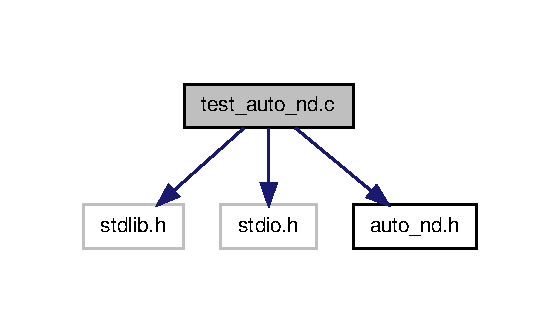
\includegraphics[width=268pt]{test__auto__nd_8c__incl}
\end{center}
\end{figure}
\subsection*{\-Fonctions}
\begin{DoxyCompactItemize}
\item 
int \hyperlink{test__auto__nd_8c_a7b26396c9888d66d997b0007e8ff1e60}{main} (int argc, char $\ast$$\ast$argv, char $\ast$$\ast$env)
\end{DoxyCompactItemize}


\subsection{\-Description détaillée}
\-Tests des \-Automates indéterministes. \begin{DoxyAuthor}{\-Auteur}
\-Gauthier \-Silvère
\end{DoxyAuthor}
\-Fichier de tests fonctionnels des automates indéterministes. 

\-Définition dans le fichier \hyperlink{test__auto__nd_8c_source}{test\-\_\-auto\-\_\-nd.\-c}.



\subsection{\-Documentation des fonctions}
\hypertarget{test__auto__nd_8c_a7b26396c9888d66d997b0007e8ff1e60}{\index{test\-\_\-auto\-\_\-nd.\-c@{test\-\_\-auto\-\_\-nd.\-c}!main@{main}}
\index{main@{main}!test_auto_nd.c@{test\-\_\-auto\-\_\-nd.\-c}}
\subsubsection[{main}]{\setlength{\rightskip}{0pt plus 5cm}int {\bf main} (
\begin{DoxyParamCaption}
\item[{int}]{argc, }
\item[{char $\ast$$\ast$}]{argv, }
\item[{char $\ast$$\ast$}]{env}
\end{DoxyParamCaption}
)}}\label{test__auto__nd_8c_a7b26396c9888d66d997b0007e8ff1e60}


\-Définition à la ligne 14 du fichier test\-\_\-auto\-\_\-nd.\-c.


\printindex
\end{document}
